\documentclass[11pt, oneside]{book}
%%% packages
\usepackage[german]{babel}
\usepackage{amsmath}
\usepackage{amssymb}
\usepackage{amsthm}
\usepackage{enumitem}
\usepackage{geometry}
\usepackage{xfrac}
\usepackage{faktor}
\usepackage{mathtools}
\usepackage{mathrsfs}
\usepackage{newclude} %no pagebreaks after \include* 
\usepackage[textsize=tiny]{todonotes}
\usepackage{xcolor}

\usepackage{graphicx}
\usepackage[hidelinks]{hyperref}
% happy proof
\usepackage{svg}
\usepackage[export]{adjustbox}

%%%% happy proof
% \happybegin for removing usual qued symbol
% \happyend to insert happy-qued instead
\newcommand\happybegin{\renewcommand{\qedsymbol}{}}
\newcommand\happyend{\hfill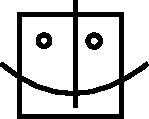
\includegraphics[width=1em]{smiley.pdf}}

\newcommand\unsure[1]{\todo[inline,linecolor=red,backgroundcolor=red!25,bordercolor=red]{#1}}

\geometry{a4paper, left = 20mm, right = 20mm, top = 30mm}

%%% commands
\newcommand{\R}{\mathbb{R}}
\newcommand{\C}{\mathbb{C}}
\newcommand{\N}{\mathbb{N}}
\newcommand{\Z}{\mathbb{Z}}
\newcommand{\K}{\mathbb{K}}
\newcommand\norm[1]{\left\lVert#1\right\rVert}
\newcommand\hnorm[1]{\hat\lVert#1\hat\rVert}

\newcommand{\B}{\mathcal{B}}

\newcommand\norms[1]{\left\lVert#1\right\rVert_\infty}
\newcommand\seq[2]{\left (#1_#2\right )_{#2\in \mathbb{N}}} %\se{f(x_n)}{n}
\newcommand\ab[1]{\left\lvert #1 \right\rvert} 
\newcommand\li[2]{\lim_{#2 \to \infty} #1_#2} %\li xn
\newcommand\lime[1]{\lim_{#1 \to\infty}} %\lime{f(x_k)}{k}
\newcommand\se[2]{\left (#1\right )_{#2\in \mathbb{N}}}
\newcommand\set[1]{\left\{#1\right\}}
\newcommand\equ[1]{\left[ #1\right]}
\newcommand\mc[1]{\mathcal{#1}}
\newcommand{\p}{\mathcal{L}}
\newcommand\ip[1]{\left\langle#1\right\rangle}
\newcommand\muq{\overset{\mu}{=}}
\newcommand\ser[2]{\sum_{#2=0}^\infty #1}

%%%%%%%%%%%%%%%%%%%%%%%%
\newcommand\normn[2]{\left\lVert#1\right\rVert_{#2}}
\newcommand{\forw}{\((\Longrightarrow)\)}
\newcommand{\backw}{\((\Longleftarrow)\)}
%%%%%%%%%%%%%%%%%%%%%%%
\newcommand{\tr}{\text{tr}}

\newcommand{\as}{{\"a}}
\newcommand{\As}{{\"A}}
\newcommand{\Os}{{\"O}}
\newcommand{\os}{{\"o}}
\newcommand{\us}{{\"u}}
\newcommand{\Us}{{\"U}}
\newcommand{\s}{{\ss}}

%%% Formatierung etc.
\theoremstyle{definition}
\newtheorem{definition}{Definition}[section]
\newtheorem{theorem}{Satz}[section]
\newtheorem{lemma}{Lemma}[section]
\newtheorem{ex}{Beispiel}[section]
\theoremstyle{remark}
\newtheorem{rem}{Bemerkung}[section]


\title{\huge{Skript Funktionalanalysis}\\ \vspace{1cm}\Large{Prof. Volkmar Liebscher SoSe2024}}
\author{\small{Jonas Harder und Jakob Kropf}}
\date{\footnotesize{Version vom \today}} 
\begin{document}
	\maketitle
	\listoftodos[Todo-Liste]
	\tableofcontents
	\chapter{Metrische R\"aume}
\section{Definitionen}

\begin{definition} \label{def_metrik}
	Eine Menge $T$, versehen mit einer Abbildung \(d: T \times T \to \R\) mit den Eigenschaften (\(s,t,u \in T\) beliebig)
	\begin{enumerate}[noitemsep]
		\item \(d(s,t)\geq 0\),
		\item \(d(s,t) = d(t,s)\)
		\item \(d(s,u) \leq d(s,t) + d(t,u)\)
		\item \(d(s,t) = 0 \iff s = t\) \label{homogen_metrik}	\end{enumerate}
	ist \textit{metrischer Raum} mit \textit{Metrik} $d$. Falls nur $(\Leftarrow)$ in \ref{homogen_metrik}. gilt, handelt es sich um eine \textit{Halbmetrik}. 
\end{definition}

\begin{ex}
	\((\R, \ab \cdot)\) ist ein metrischer Raum.
\end{ex}
\begin{ex}
\((\C, \ab \cdot )\) ist ein metrischer Raum. 
\end{ex}
\begin{ex}
	\((\R^n, d_i)\) mit \(i \in \{1,2,\infty\}\) sind metrische R\as ume, wobei f\us r \(x,y \in \R\)
	\[d_1 := \sqrt{\sum_{i=1}^n  (x_i -y_i) },\;\;\;\; d_2 := \sqrt{\sum_{i = 1}^n (x_i - y_i)^2}, \;\;\;\; d_\infty := \max \{\ab{x_i - y_i}\vert i: 1,\ldots, n\}\]
\end{ex}
\begin{definition}
	Sei \(X,d\) ein metrischer Raum. Dann definieren wir die offene bzw. abschlossene Kugel um \(x\in X\)wie folgt.
	\[K_\nu (x) := \{y \in X \vert d(x,y) \leq \nu\} \;\;\;\; \overline{K_\nu(x)} := \{y \in X \vert d(x,y) \leq \nu \}\]
	Weiterhin ist \(U \text{ eine Umgebung von } x \iff \exists \nu > 0: K_\nu(x) \subseteq U\).
\end{definition}

\section{Konvergenz und Stetigkeit}
\begin{definition}
	Eine Folge \(\seq x n\)  in einem metrischen Raum $X$ hei\s t \textit{konvergent} gegen $x \in X$  (bez. $\li tn  = t$), falls 
	\[\forall \varepsilon > 0 \;\exists N \in \N \forall n \geq N: d(x_n, x) \leq \varepsilon \;\;.\]
\end{definition}
\begin{theorem}
	Der Limes einer konvergenten Folge ist eindeutig bestimmt. 
\end{theorem}
\begin{theorem}
	Jede Teilfolge einer konvergenten Folge ist konvergent und hat den gleichen Grenzwert.
\end{theorem}

\begin{definition}
	Sei \(f: (X_1, d_1) \to (X_2, d_2)\) eine Abbildung zwischen metrischen R\as umen. Dann hei\s t $f$ \textit{stetig an der Stelle} $x_0 \in X_1$, falls
	\[\forall \varepsilon > 0\;\exists \delta > 0: d_1(x, x_0) < \delta \implies d_2(f(x), f(x_0)) < \varepsilon\]
\end{definition}

\begin{theorem}
	Sei \(f: (X_1, d_1) \to (X_2, d_2)\) eine Abbildung zwischen metrischen R\as umen. Dann sind folgende Bedingungen \as quivalent:
	\begin{enumerate}[noitemsep]
		\item $f$ ist stetig an $x_0$
		\item $\forall \seq x n \text{ mit }x_n \in X_1 \forall n \in \N : \li x n = x_0 \in X_1 \implies \lim_{n \to \infty} f(x_n) = f(x_0)$ 
	\end{enumerate}
\end{theorem}
\begin{theorem}
	Seien \(f: X_1 \to X_2\), \(g: X_2\to X_3\) stetige Abbildungen zwischen metrischen R\as umen. Dann ist die Verkn\us pfung \(g \circ f: X_1 \to X_3\) stetig. 
\end{theorem}

\section{Offene und abgeschlossene Mengen}
\begin{definition}
	Sei \((X,d)\) ein metrischer Raum, dann hei\s t 
	\begin{enumerate}[noitemsep]
		\item \(G \subseteq X \) offen \(:\iff \forall x \in G\; \exists \nu > 0: K_\nu(x) \subseteq G\)
		\item \(F \subseteq X\) abgeschlossen \(:\iff \forall \seq x n \text{ mit } x_n \in F \;\forall n \in \N: \li xn = x \implies x \in F\)
		\item $S \subseteq X$ liegt dicht in $X$ \(:\iff \forall x \in X \;\exists \seq  s n, s_n \in S: \li sn = x \)
	\end{enumerate}
\end{definition}

\begin{definition}
	Ein metrischer Raum \((X, d)\) hei\s t \textit{separabel}, wenn es eine h\os chstens abz\as hlbare Teilmenge \(S\subseteq X\) gibt, die in diesem Raum dicht liegt.
\end{definition}
\begin{ex}
	Der Banachraum 
	\[l^\infty(\N) := \{\seq an \vert a_n \in \R, \seq a n \text { beschr\as nkt}\} \;\; \text{ mit } d_\infty(\seq an, \seq bn) = \sup_{n\in \N} \ab{a_n - b_n}\] 
	ist nicht separabel.
\end{ex}

\begin{theorem}
	\label{stetig_abb}Sei \(f: (X_1, d_1) \to (X_2, d_2)\) eine Abbildung zwischen metrischen R\as umen. Dann sind \as quivalent:
	\begin{enumerate}[noitemsep]
		\item $f$ ist stetig.
		\item \(\forall G \subseteq X_2: G \text{ offen} \implies f^{-1}(G)\) offen.
		\item \(\forall F \subseteq X_2: F \text{ abgeschlossen} \implies f^{-1}(F)\) abgeschlossen.
	\end{enumerate}
\end{theorem}

\begin{rem}
	Aus Satz \ref{stetig_abb} folgt: 
	\(K_\varepsilon(x) \text{ offen, da } K_\varepsilon(x) = d(x, \cdot)^{-1}((-\infty, \varepsilon))\).
\end{rem}

\section{Vollst\as ndigkeit}

\begin{definition}
	Sei $(X,d)$ ein metrischer Raum, dann hei\s t $\seq xn$ mit $\forall n \in \N: x_n \in X$ \textit{Cauchyfolge}, falls:
	\[\forall \varepsilon > 0 \; \exists N \in \N \; \forall n, m \geq N: d(x_n, x_m) < \varepsilon\]
\end{definition}

\begin{theorem}
	Jede konvergente Folge $\seq x n$ in einem metrischen Raum $(X, d)$ ist eine Cauchy-Folge.
\end{theorem}

\begin{definition}
	Ein metrischer Raum $(X, d)$ hei\s t vollst\as ndig, falls jede Cauchyfolge konvergiert.
\end{definition}

\begin{ex}
	\((\R, \ab \cdot)\) und \(\C, \ab \cdot\) sind vollst\as ndige metrische R\as ume. 
\end{ex}

\begin{ex}
	Die metrischen R\as ume  \((\R^n, f_p)\) mit \(p \in [1, \infty]\) sind vollst\as ndig.
\end{ex}

\begin{theorem}
	Sei \((X, d)\) ein vollst\as ndiger metrischer Raum. Dann gilt: 
	\[ Y \subseteq X \text{ vollst\as ndig} \iff Y \text{ abgeschlossen.}\]
\end{theorem}

\begin{theorem}
	Sei \((X_1,d_1)\) ein metrischer Raum \((X_2, d_2)\) ein vollst\as ndiger metrischer Raum sowie \(\varphi: X_1 \to X_2\) isometrisch. Dann gibt es genau eine isometrisches \(\hat\varphi: X_1\to X_2\) mit \(\hat\varphi\vert_S = \varphi\).
	\label{vollst_isometrie}
\end{theorem}
\begin{proof}
	Sei \(x\in X_1\), dann gibt es eine Folge \(\seq xn\) mit \(\forall n \in \N: x_n \in S\) und \(\li xn = x\). Somit ist \(\seq xn\) insbesondere eine Cauchyfolge. Folglich ist auch \((\varphi(x_n))_{n\in\N}\) eine Cauchyfolge und mit der Vollst\as ndigkeit von $X_2$ gilt
	\[\exists y\in X_2: \lime n \varphi(x_n) = y:= \hat\varphi(x)\;.\]
	Wir setzen also f\us r solche Folgen \[\hat\varphi\left(\li x n\right) := \lime n \varphi(x_n)\;.\]
	Zeige nun \(\hat \varphi\) ist wohldefiniert. Sei eine weitere Folge \(\seq yn\) gegeben mit \(\forall n \in \N: y_n \in S\) und \(\li yn = x\). Es folgt:
	\[d_2(\varphi(x_n), \varphi(y_n)) = d_1(x_n, y_n) \overset{n\to\infty}{\longrightarrow} d_1(x,x) = 0 \implies \lime n \varphi(y_n) = y\;.\]
	Somit ist $\hat\varphi$ in der Tat wohldefiniert. Weiterhin gilt \(\hat\varphi\vert_S = \varphi\), denn wir w\as hlen f\us r \(x \in S\) die Folge $\se x n$, somit gilt
	\[ \hat \varphi\left(\li x n \right) = \hat\varphi(x) = \lime n \varphi(x_n) = \lime n \varphi(x) = \varphi(x)\;.\] 
	Zeige nun \(\hat\varphi\) ist eine Isometrie. Seien dazu \(x,y\in X\) mit  $\seq xn$, $\seq yn$ Folgen in $S$, wobei $\li x n = x$, $\li y n = y$. Somit
	\[d_2(\hat\varphi(x), \hat\varphi(y)) = \lime n d_2(\varphi(x_n), \varphi(y_n)) = \lime n d_1(x_n, y_n) = d(x,y) \;.\] 
\end{proof}

\begin{theorem}
	Sei $(X,d)$ ein metrischer Raum. Dann gibt es einen vollst\as ndigen metrischen Raum $(\hat X, \hat d)$ (bez. Vervollst\as ndigung von $X$) und eine Isometrie \(\varphi: X \to \hat X\) (d. h. \(\forall x, y \in X: d(x,y) = \hat d (\varphi(x), \varphi(y))\)), sodass das Bild $\varphi(X)$ dicht in $\hat X$ ist. Haben $(\tilde X, \tilde d)$ und $\tilde \varphi$ die gleiche Eigenschaft, so gibt es eine Bijektion \(\psi: \hat X \to \tilde X\) mit \(\tilde \varphi = \psi \circ \varphi\).
	\label{vervollst_mR}
\end{theorem}
\begin{proof}
	Definiere die Menge aller Cauchyfolgen in $X$ durch 
	\[\hat X_0 := \{\seq x n \vert \forall n \in \N: x_n \in X, \; \seq x n \text{ Cauchyfolge}\}.\]
	Definiere weiterhin eine \As quivalenzrelation $\sim$ auf $\hat X_0$ mit 
	\[\seq xn \sim \seq yn :\iff \lim_{n\to\infty} d(x_n, y_n) = 0\;.\]
	Wir setzen $\hat X$ als die Menge aller \As quivalenzklassen an, d. h.
	\[\hat X = \faktor{\hat X_0}{\sim} = \{\equ{\seq xn} \vert \seq xn \in \hat X_0\} \text { wobei } \equ{\seq xn} = \{\seq yn \vert \seq xn \sim \seq yn\}\;. \]
	Nun konstruieren wir die Metrik $\hat d: \hat X \times \hat X \to  [0, \infty) $, wobei f\us r \(\equ{\seq xn}, \equ{\seq yn} \in \hat X\) gilt
	\[\hat d(\equ{\seq xn}, \equ{\seq yn}) = \lim_{n, m\to \infty} d(x_n, y_m) \iff \forall \varepsilon > 0 \;\exists N, M \in \N\;\forall n \geq N \; \forall m \geq M: d(x_n, y_m) < \varepsilon\; . \]
	Zeigen nun, dass $\hat d$ wohldefiniert. Seien $\seq {x'}{n}, \seq{y'}{n} \in \hat X_0$ mit \(\seq xn \sim \seq{x'}{n}, \seq yn \sim \seq{y'}{n}\), dann nach Definition
	\[\lim_{n \to \infty}d(x_n, x'_n) = \lim_{n\to\infty}d(y_n, y'_n) = 0\;.\]
	Anwenden der Dreiecksungleichung ergibt
	\begin{align*}
		& d(x_n, y_n) \leq d(x_n, x'_n) + d(x'_n, y'_n) + d(y'_n, y_n)\\
		&d(x'_n, y'_n) \leq d(x'_n, x_n) + d(x_n, y_n) + d(y_n, y'_n) \; .
	\end{align*}
	Somit
	\[\ab{d(x_n,y_n) - d(x'_n, y'_n)} \leq d(x_n, x'_n) + d(y_n, y'_n) \to 0\;.\]
	Da $(d(x_n, y_n))$ und $(d(x'_n, y'_n))$ konvergent, folgt
	\[\lim_{n, m\to\infty} d(x_n, y_m) = \lim_{n',m'\to\infty} d(x'_{n'}, y'_{m'})\]
	und somit ist $\hat d$ wohldefiniert. Nun gilt nach Def. \ref{def_metrik} zu zeigen, dass $\hat d$ eine Metrik auf $\hat X$ ist. Wir zeigen hier nur die Dreiecksungleichung:
	\begin{align*}
		 \lim_{n, m \to \infty} d(x_n, y_m) &\leq \lim_{k\to\infty}\lim_{n,m \to\infty} d(x_n, z_k) + d(z_k, y_m) \iff \\
		 \hat d(\equ{\seq xn},\equ{\seq yn}) &\leq \hat d(\equ{\seq xn}, \equ{\seq zk}) + \hat d(\equ{\seq zk}, \equ{\seq yn}) \;.
	\end{align*}
	Setze nun
	\(\varphi: X \to \hat X, \;, x \mapsto \equ{(x)_{n\in\N}}\), dies ist offensichtlich eine Isometrie. Zeigen nun, dass $\varphi(X)$ dicht in $\hat X$. Sei $\equ{\seq xn} \in \hat X$. Nach Voraussetzung ist $\seq xn$ eine Cauchyfolge, d. h. $\exists N_0 \in \N$ sodass \(\forall m,n \geq  N_0: d(x_m, x_n) < \varepsilon \). Somit \(\hat x_{N_0} := \equ{(x_{N_0})_{n \in \N}} = \varphi(x_{N_0}) \in \varphi(X)\) und
	\[\hat d\left (\equ{\seq xn}, \hat x_{N_0} \right) = \lim_{n\to\infty} d(x_n, x_{N_0})< \varepsilon\; .\]
	Somit \(\hat x_{N_0} \in K_\varepsilon (\equ{\seq xn}) \cap \varphi(X)\) und folglich ist \(\varphi(X)\) dicht in $\hat X$.  Nun gilt zu zeigen, dass $(\hat X, \hat d)$ vollst\as ndig ist. Zeige daf\us r zun\as chst folgendes Lemma.
	\begin{lemma}
		Sei \(X,d\) metrischer Raum, $S\subseteq X$ dicht in $X$, sodass jede Cauchyfolge in $S$ in $X$ konvergiert. Dann ist X vollst\as ndig.\label{vervollst_lemma}
	\end{lemma}
	\begin{proof}
		Sei $\seq xn$ eine Cauchyfolge in $X$. Da $S$ dicht in $X$ gilt
		\[\forall n \in \N \;\exists y_n \in S: d(x_n, y_n) < \sfrac 1n \;.\]
		Somit ist \(\seq yn\) auch eine Cauchyfolge in $S$, da
		\[d(y_m, y_n) \leq d(y_m, x_m) + d(x_m, x_n) + d(x_n, y_n) < \sfrac 1m + d(x_m, x_n) + \sfrac 1n \;.\]
		Nach Annahme existiert $\li yn =: x \in X$. Da
		\[d(x_n, x) \leq d(x_n, y_n) + d(y_n, x) < \sfrac 1n + d(y_n, x)\]
		folgt in der Tat \(\li xn = x\).
	\end{proof}
	Nach Lemma \ref{vervollst_lemma} g. z. z., dass jede Cauchyfolge in \(\varphi(X) \) in $\hat X$ konvergiert. Sei $\seq{\hat x}{k}$ Cauchyfolge in $\varphi(X)$, d. h. \(\hat x_k := (x_k, x_k,\ldots)\). Da $\varphi$ eine Isometrie, ist $\seq xk$ eine Cauchyfolge in $X$ durch 
	\[\forall m, n \in \N: d(x_n, x_m) = \hat d(\hat x_n, \hat x_m) \;.\]
	Somit \(\seq xk \in \hat X_0\), \(\equ{\seq xk} \in \hat X\). Sei $\varepsilon >0$, dann $\exists N \in \N$ mit \(\forall k, n \geq N: d(z_k, z_n) < \varepsilon\). Somit gilt \(\forall k \geq N\):
	\[\hat d(\hat x_k, \hat x) = \lim_{n\to\infty} d(z_k, z_n) < \varepsilon \;.\]
	Folglich konvergiert $\seq{\hat x}{k}$ gegen $\hat x \in \hat X$ und $\hat X$ ist vollst\as ndig.
	Betrachte nun \((\tilde X, \tilde d)\) sowie \(\tilde \varphi\) mit den gleichen Eigenschaften. Wir definieren 
	\[\psi_0: \varphi(X) \to \tilde X, \;\; \psi_0(\varphi(x)) = \tilde\varphi(x)\;.\]
	Dies ist eine Isometrie, da f\us r $x,y \in X$ gilt 
	\[\tilde d\left(\psi_0(\varphi(x)), \psi_0(\varphi(y))\right) = \tilde d(\tilde\varphi(x), \tilde\varphi(y)) = d(x,y) = \hat d(\varphi(x), \varphi(y))\;.\]
	Nach Satz \ref{vollst_isometrie} existiert eine eindeutige Erweiterung \(\psi: \hat X \to \tilde X\) Isometrie mit \(\psi\vert_{\varphi(X)} = \psi_0\). Da $\psi_0$ als Isometrie injektiv ist, g. z. z. $\psi_0$ ist surjektiv. Sei also \(z \in \tilde X\), dann wegen der Dichtheit von $\tilde\varphi(X)$
	\[\exists \seq xn, \; \forall n \in \N\; x_n \in X: \lime n \tilde\varphi(x_n) = z\;.\]
	Somit  \( \seq xn\) Cauchyfolge \( \implies \se{\varphi(x_n)}{n} \) Cauchyfolge. Da $\hat X$ vollst\as ndig
	\[\exists w \in \hat X: \lime n \varphi(x_n) = w\;.\]
	Da $\psi$ eine Isometrie ist folgt schlie\s lich \(\lime n \psi(\varphi(x_n)) = \psi(w) = z\) und somit ist $\psi$ bijektiv.
\end{proof}

\section{Kompaktheit}
\begin{definition}
	Ein metrischer Raum \((X, d)\) hei\s t \textit{kompakt}, wenn jede offene \Us berdeckung eine endliche Teil\us berdeckung besitzt. D. h., wenn $(G_i)_{i\in I}$ eine Famile offener Mengen, mit \(X = \bigcup_{i\in I} G_i\), dann existieren endlich viele \(G_{i_1},\ldots, G_{i_n}\) mit \(X = \bigcup_{k=1}^n G_{i_k}\).
\end{definition}
\begin{theorem}
	Sei \(X ,d\) metrischer Raum, \(K\subseteq X\) kompakt. Dann ist $K$ beschr\as nkt und abgeschlossen (Umkehrung gilt i. A.nicht).\label{kompakt_beschr_abg}
\end{theorem}
\begin{theorem}
	Sei \(X,d\) metrischer Raum. Dann gilt
	\[X \text{ kompakt}\iff \forall \seq xn \exists \left(x_{n_k}\right)_{k\in\N} \text{ Teilfolge } \exists y \in X: \lime k x_{n_k} = y\]
\end{theorem}
\begin{theorem}[Heine-Borel]
	Betrachte die metrischen R\as ume \((\R^n, d_p)\) mit $p\in[1,\infty]$. Dann ist \(X\subseteq \R^n\) kompakt \(\iff X\) beschr\as nkt und abgeschlossen.
\end{theorem}
\begin{definition}
	Sei \((X,d)\) metrischer Raum. Dann hei\s t \(Y\subseteq X\) totalbeschr\as nkt falls
	\[\forall \varepsilon > 0 \;\exists M \in \N\;\exists x_1,\ldots, x_M \in Y: Y \subseteq \bigcup_{i=1}^M K_\varepsilon (x_i)\]
\end{definition}
\begin{theorem}
	Sei \(X, d\) ein vollst\as ndiger metrischer Raum, \(Y\subseteq X\). Dann ist $Y$ kompakt $\iff Y$ abgeschlossen und total beschr\as nkt. 
\end{theorem}
\begin{proof}
	 \((\Longrightarrow)\)\\
	 Sei $Y$ kompakt. $Y$ abgeschlossen folgt aus Satz  \ref{kompakt_beschr_abg}. Zeige nun die totale Beschr\as nktheit, sei $\varepsilon>0$ daf\us r fixiert. Dann gilt offensichtlich
	 \[Y \subseteq \bigcup_{y\in Y} K_\varepsilon(y) \overset{\text{$Y$ kompakt}}{\implies}\exists y_1,\ldots,y_M: Y \subseteq \bigcup_{i=1}^M K_\varepsilon(y_i)\]
	 Somit ist $Y$ total beschr\as nkt. \\
	 \((\Longleftarrow)\)\\
	 Sei $Y\subseteq X$ abgeschlossen und total beschr\as nkt und sei \(\seq xn\) eine Folge aus $Y$. Es g. z. z., dass \(\seq xn\) eine in $Y$ konvergente Teilfolge besitzt. 
	 Wir nutzen die totale Beschr\as nktheit zur Konstruktion der Teilfolge (TF).
	 \begin{align*}
	  \varepsilon = 1: \; &\exists \set{y^1_i}_{i = 1,\ldots, M_1}, \; Y \subseteq \bigcup_{i=1}^{M_1} K_1\left(y^1_i\right) \implies \exists \text{ TF } \se{x_{n^1_k}}{k} \exists i_1 \in \set{1,\ldots,M_1} \forall k \in \N: x_{n^1_k} \in K_1\left(y_{i_1}^1\right) \\
	 	 \varepsilon = \frac{1}{2}: \; &\exists \set{y^2_i}_{i = 1,\ldots, M_2}, \; Y \subseteq \bigcup_{i=1}^{M_2} K_{\sfrac12}\left(y^2_i\right) \implies \exists \text{ TTF } \se{x_{n^2_k}}{k} \exists i_2 \in \set{1,\ldots,M_2}\\
	 	 & \forall k \in \N: x_{n^2_k} \in K_1\left(y_{i_1}^1\right) \cap K_{\sfrac12}\left(y_{i_2}^2\right)
	 \end{align*}
	 Diese Konstruktion l\as sst sich nun auf $l$ Schritte erweitern.
	 \begin{align*}
	 	 \varepsilon = 2^{-l}: \; &\exists \set{y^l_i}_{i = 1,\ldots, M_l}, \; Y \subseteq \bigcup_{i=1}^{M_l} K_{2^{-l}}\left(y^l_i\right) \implies \exists \text{ TT\ldots TF } \se{x_{n^l_k}}{k} \exists i_l \in \set{1,\ldots,M_l}\\
	 	& \forall k \in \N: x_{n^l_k} \in K_1\left(y_{i_1}^1\right) \cap K_{\sfrac12}\left(y_{i_2}^2\right) \cap \ldots \cap K_{2^{-(l-1)}}\left(y_{i_{l-1}}^{l-1}\right) \cap K_{2^{-l}}\left(y_{i_{l}}^l\right)
	 	\end{align*}
	 Nach Konstruktion ist \(\se{x_{n_k}^k}{k}\) Teilfolge von \(\seq xn\) und f\us r \(k, k'\geq l\) gilt
	 \[x_{n_k}^k,\; x_{n_{k'}}^{k'} \in K_{2^{-l}}\left(y_{i_{l}}^l\right) \implies d\left(x_{n_k}^k, x_{n_{k'}}^{k'}\right) < 2^{-(l-1)}\;.\]
	 Folglich ist \(\se{x_{n_k}^k}{k}\) eine Cauchyfolge und da $X$ nach Voraussetzung vollst\as ndig, gilt 
	 \[\exists z\in X: \lime k x_{n_k}^k = z \;.\]
	 Da $Y$ abgeschlossen, gilt insbesondere \(z\in Y\) und folglich $Y$ kompakt.
	\end{proof}
	 \begin{ex}
	 	Betrachte 
	 	\[C[0,1] := \set{f:[0,1] \to \R \;\vert\; f\text{ stetig}}, \;\; \norms\cdot , \text{ f\us r } f, g \in C[0,1]: d(f,g) = \max \set{\ab{f(t)- g(t)}\;\vert\; t\in[0,1]}\;\;\]
	 	Dann gilt $Y\subseteq C[0,1]$ ist kompakt $\iff Y$punktweise beschr\as nkt, d. h. 
	 	\[\exists c>0 \;\forall f \in Y \;\forall t \in [0,1]: \ab{f(t)} \leq c\]
	 	und $Y$ gleichgradig stetig, d. h. 
	 	\[\forall \varepsilon > 0\; \exists \delta > 0 \;\forall f \in Y\;\forall s, t \in [0,1]: \ab{t-s} < \delta \implies \ab{f(t) - f(s)} < \varepsilon \;.\]
	 \end{ex} 
	 
	 \begin{theorem}
	 	Sei \((X_1, d_1)\) ein kompakter metrischer Raum, \((X_2, d_2)\) ein metrischer Raum, sowie \(f:X_1 \to X_2\) stetig. Dann ist \(f(X_1)\) kompakt.
	 \end{theorem}
	 \begin{rem}
	 	Falls $X_2 = \R$, dann existieren nach dem Satz von Weierstra\s{} \(x_+, x_- \in X_1\) mit \(f(x_+) = \sup f(X_1)\) und \(f(x_-) = \inf f(X_1)\).
	 \end{rem}
	 
	 \begin{theorem}
	 		Sei \((X_1, d_1)\) ein kompakter metrischer Raum, \((X_2, d_2)\) ein metrischer Raum, sowie \(f:X_1 \to X_2\) stetig. Dann ist $f$ gleichm\as \s ig stetig, d. h. 
	 		\[\forall \varepsilon > 0 \;\exists \delta > 0 \;\forall x,y \in X_1: d_1(x,y) < \delta \implies d_2(f(x), f(y)) < \varepsilon\;.\]
	 		
	 \end{theorem}

	\chapter{Ma\s{}- und Integrationstheorie}
\section{Grundlegende Konstruktionen}
\begin{definition}
	Sei \(\Omega \neq \emptyset\). Dann hei\s t \(\mc F \subseteq \mc P (\Omega)\)  $\sigma$-Algebra, falls
	\begin{enumerate}[noitemsep]
		\item \(\Omega \in \mc F\)
		\item \(\forall A \subseteq \mc P(\Omega): A\in \mc F \implies A^C \in \mc F\)
		\item \(\forall \seq An,\; \forall n\in \N\; A_n \in \mc F: \bigcup_{n\in\N}\in\mc F\)
	\end{enumerate}
	Bezeichne \((\Omega, \mc F)\) als messbaren Raum.
\end{definition}
\begin{rem}
	Sei \((X, d)\) ein metrischer Raum, dann ist die $\sigma$-Algebra \(\mc B(X)\) der Borelmengen die kleinste $\sigma$-Algebra, die alle offenen Mengen von $X$ enth\as lt. Bez. \(\mc B(\R) =: \mc B\) und \(\mc B(\R^n) = \mc B^n\).
\end{rem}
\begin{definition}
	Sei \(\Omega, \mc F\) ein messbarer Raum. Dann ist \(\mu: \mc F \to [0,\infty]\) ein Ma\s{}, falls
	\begin{enumerate}[noitemsep]
		\item \(\mu(\emptyset) = 0\)
		\item \(\forall \seq An, \; \forall n\in\N: A_n \in \mc F, \; \forall i, j \in \N, i\neq j: A_i\cap A_j = \emptyset: \mu\left( \cup_{n\in\N} A_n\right) = \sum_{n\in\N} \mu(A_n)\)
	\end{enumerate}
	Wir bezeichnen \((\Omega, \mc F, \mu)\) als Ma\s raum.
\end{definition}
\begin{definition}
	Sei \((\Omega, \mc F, \mu)\) ein Ma\s raum. Das Ma\s{} $\mu$ wird als $\sigma$-endlich bezeichnet, falls gilt
	\[\exists A_1, A_2,\ldots \in \mc F,\; A_1\subseteq A_2\subseteq \ldots \;\text{ mit }\; \forall n \in \N: \mu(A_n) < \infty \text{ und } \bigcup_{n\in \N}A_n = \Omega\;.\]
\end{definition}
\begin{definition}
	Sei \((\Omega, \mc F, \mu)\) ein Ma\s raum. Ein Ma\s{} \(\nu: \mc F \to [0,\infty]\) hei\s t absolut stetig bzgl. \(\mu\) (bez. \(\nu \ll \mu\)), falls 
	\[\forall A\in \mc F: \mu(A) = 0 \implies \nu(A) = 0\;.\]
\end{definition}

\begin{ex}
	Sei \(\Omega\) beliebig und \(\mc F = \mc P(\Omega)\). Dann k\os nnen wir das Z\as hlma\s{}  $\mu$ definieren mit \(A \in \mc P(\Omega)\)
	\[\mu(A) = \begin{cases}\ab{A} & $A$ \text{ endlich}\\ \infty & \text{sonst}\end{cases} \] 
	Dabei ist $\Omega$ meist abz\as hlbar, z. B. \(\Omega = \N\) oder \(\Omega = \Z\)
\end{ex}

\begin{ex}
	Sei \(\Omega = \R^n\) und \(\mc F = \mc B ^n\). Dann definieren wir das Lebesgue-Ma\s{} $l^n$ mit 
	\[l^n\left(\bigtimes_{i=1}^n [a_i, b_i)\right) = \prod_{i=1}^n (b_i -a_i)\;.\]
	F\us r $l=1$ gilt damit insbesondere \(l^1([a,b)) =: l([a,b)) = b-a\).
\end{ex}

\section{Integration}
\begin{definition}
	Sei \((\Omega, \mc F)\) ein messbarer Raum, \(f:\Omega\to \C\) hei\s t messbar (bez. \(f\in \mc M (\Omega, \mc F, \C)\)), falls
	\[\forall r > 0, z \in \C: f^{-1}(K_r(z)) \in \mc F \;\;[\iff \forall U \in \mc B(\C) : f^{-1}(U) \in \mc F]\;.\]
	Analog ist \(f:\Omega \to \R\) messbar (bez. \(f \in \mc M (\Omega, \mc F, \R)\)), falls
	\[\forall U \in \mc B(\R): f^{-1}(U) \in \mc F\]
\end{definition}
\begin{rem}
	Wir bezeichnen weiterhin \(\mc M(\Omega, \mc F, [0,\infty)) := \mc M_+(\Omega)\).
\end{rem}
\begin{rem}
	Sei \(\Omega, \mc F\) ein messbarer Raum, \(f: \Omega \to \R\). Dann ist $f$ messbar 
	\[\iff \forall c\in \R: \set{f > c} := \set{x\in \Omega \vert f(x) > c} \in \mc F\;.\]
\end{rem}

\begin{definition}
	Sei $A$ eine Menge. Eine Funktion der Form
	\[1_A(\omega)\begin{cases}1 & \omega \in A \\ 0 & \omega \not\in A\end{cases}\]
	hei\s t \textit{Indikatorfunktion} der Menge $A$.
\end{definition}
\begin{theorem}[Integral f\us r nichtnegative, messbare Funktionen]
	Sei \((\Omega, \mc F, \mu)\) ein Ma\s raum. Dann gibt es genau eine Abbildung \(\varphi: \mc M_+(\Omega) \to [0,\infty]\) mit:
	\begin{enumerate}
		\item \(\forall A \in \mc F: \varphi(1_A) = \mu(A)\)
		\item \(\forall f, g \in \mc M_+(\Omega), \lambda \in [0,\infty]: \varphi(\lambda f + g) = \lambda\varphi(f) + \varphi(g)\) \label{linearitaet_integral}
		\item \(\forall \seq f n,\; \forall n \in \N f_{n+1} \geq f_{n} \geq 0: \varphi(\li fn) = \lime n \varphi(f_n)\) \label{Beppo_Levi}
	\end{enumerate}
	Wir schreiben \(\varphi(f)  =: \int f d\mu =: \int f(\omega) d(\omega) =:\int f(\omega) \mu(d \omega)\).
\end{theorem}
\begin{rem}
	\ref{Beppo_Levi}. ist auch als Satz von Beppo Levi \us ber monotone Konvergenz bekannt.
\end{rem}
\begin{rem}
	Wir k\os nnen in \ref{linearitaet_integral}. \(\lambda \in [0, \infty]\) w\as hlen unter Beachtung, dass auf den erweiterten reellen Zahlen \(\bar\R := \R \cup \set{-\infty, \infty}\) gilt:
	\[0\cdot (\pm \infty) = (\pm \infty) \cdot 0 : = 0 \;\text{ und }\; (+\infty) + (-\infty) = (-\infty) + (+\infty) = 0\;.\]
\end{rem}
\begin{definition}[Integral f\us r messbare Funktionen]
	Sei \((\Omega, \mc F, \mu)\) ein Ma\s raum, \(f\in \mc M(\Omega, \mc F, \R)\). Dann definieren wir
	\[f^+ := \max\set{f,0}, \;\; f^- := \max\set{-f,0} \implies f = f^+ - f^- \text{ und } \ab{f} = f^+ + f^-\;.\]
	Somit erhalten wir als Definition f\us r das Integral (f\us r integrierbare Funktionen, siehe Def. \ref{integrierbare_funkt}):
	\[\int f d\mu : = \int f^+ d\mu - \int f^- d\mu\;.\]
	Sei nun \(f\in \mc M(\Omega, \mc F,\C)\), dann folgt \(\Re(f), \Im(f) \in \mc M (\Omega, \mc F, \R)\). Somit k\os nnen wir definieren:
	\[\int f d\mu := \int \Re(f) d\mu + i \cdot \int \Im(f) d\mu\;.\]
\end{definition}
\begin{definition}
		\label{integrierbare_funkt}
		Sei \((\Omega, \mc F, \mu)\) ein Ma\s raum. Dann bezeichnen wir $f: \Omega \to \C$ als ($\mu$-)integrierbar, falls $f\in \p^1$, wobei gilt
		\[\p^1(\Omega, \mc F, \mu, \C) := \set{f\in \mc M(\Omega,\mc F, \C)\Big\vert \int \ab{f} d\mu < \infty}\;.\]
		Wir schreiben kurz auch \(\p^1(\Omega, \mc F, \mu)\).
\end{definition}
\begin{rem}
	Analog definiert man \(\p^1(\Omega, \mc F, \mu, \R)\). Somit:
	\[\int \cdot \;d\mu : \p^1(\Omega, \mc F, \mu, \R\;[\C]) \to \R \;[\C]\]
\end{rem}
\begin{rem}
	F\us r \(f:\Omega \to \C\) gilt insbesondere \(\ab{f} \geq \Re(f)\), \(\ab{f} \geq \Im(f)\), d. h. das Integral ist wohldefiniert.
\end{rem}
\begin{theorem}
	Seien \(f,g\in \mc \p^1(\Omega, \mc F, \mu)\) sowie eine Folge \(\seq fn, \forall n \in \N :f_n \in \p^1(\Omega, \mc F, \mu)\) sowie \(\lambda \in \C\). Dann gilt:
	\begin{enumerate}
		\item \(\ab{\int f d\mu} \leq \int \ab{f} d\mu\)
		\item \(\int \lambda f + g d \mu = \lambda \int f d \mu + \int g d \mu\)
		\item \(\mu\left(\set{\omega\in \Omega\vert f(\omega) \neq g(\omega)}\right) = 0 \implies \int f d\mu = \int g d \mu \implies \int \ab{f-g} d \mu = 0\)
		\item \(\mu\left(\set{\omega\in \Omega\vert \ab{f(\omega)} = \infty}\right)\) = 0
		\item \(\exists h: \Omega \to [0,\infty],\; h \in \p^1(\Omega, \mc F,\mu)\; \forall n \in \N: \ab{f_n} \leq h \text{ und } \li fn = f \implies \int f d \mu = \int \li fn d \mu = \lime n \int f_n d\mu\) \label{Lebesgue}
	\end{enumerate}
\end{theorem}
\begin{rem}
	\ref{Lebesgue}. ist auch als Satz von Lebesgue \us ber die majorisierte Konvergenz bekannt.
\end{rem}

\begin{definition}
	Seien \((\Omega_1, \mc A)\), \((\Omega_2, \mc B)\) Ma\s r\as ume. Dann hei\s t die kleinste \(\sigma\)-Algebra auf \(\Omega_1 \times \Omega_2\), die die Menge 
	\[\set{A\times B \;\vert\; A\in \mc A,\; B\in\mc B}\]
	enth\as lt, Produkt-$\sigma$-Algebra. Wir bezeichnen diese mit \(\mc A \otimes \mc B\).
\end{definition}

\begin{theorem}[Produktma\s]
	Seien \((\Omega_1, \mc A, \mu)\) und \((\Omega_2, \mc B, \nu)\) $\sigma$-endliche Ma\s r\as ume. Dann existiert genau ein Ma\s{} \(\mu\otimes\nu: A\otimes B \to [0,\infty]\) mit 
	\[\forall A \in \mc A, B\in\mc B: (\mu \otimes \nu)(A\times B) = \mu(A) \nu(B)\;.\]
	Dabei ist \(\mu\otimes \nu\) $\sigma$-endlich und wir bezeichnen dies als Produktma\s{} von \(\mu\) und \(\nu\).
\end{theorem}

\begin{theorem}[Satz von Fubini]
	\label{Fubini}
	Seien die Ma\s r\as ume wie f\us r das Produktma\s{} definiert. Sei weiterhin \(f\in \mc L^1(\mu\otimes \nu)\), dann gilt
	\[\int_{\Omega_1\times \Omega_2} f(x,y) \mu \otimes \nu(d(x,y)) = \int_{\Omega_2}\left(\int_{\Omega_1} f(x,y) \mu (dx)\right) \nu(dy) = \int_{\Omega_1}\left(\int_{\Omega_2} f(x,y) \nu (dy)\right) \mu(dx)\;.\]
\end{theorem}

\begin{definition}
	Sei \((\Omega, \mc F, \mu)\) ein Ma\s raum, \(\nu: \mc F \to [0,\infty]\) ein Ma\s{}. Dann besitzt $\nu$ eine Dichte bzgl. $\mu$, falls
	\[\exists f:\Omega \to [0,\infty) \text{ messbar}: \forall A \in \mc F: \nu(A) = \int_A f d\mu\;.\]
\end{definition}

\begin{theorem}[Satz von Radon-Nikodym] \label{radon_nikodym} Sei \((\Omega, \mc F, \mu)\) ein $\sigma$-endlicher Ma\s raum und \(\nu: \mc F \to [0,\infty]\) ein Ma\s{} mit \(\nu \ll\mu\). Dann besitzt \(\nu\) eine Dichte bzgl. $\mu$.
\end{theorem}




	\chapter{Normierte R\as ume}
\section{Definitionen}
\begin{rem}
	Wir betrachten hier Vektorr\as ume \us ber den K\os rpern \(\K = \R\) oder \(\K = \C\).
\end{rem}
\begin{definition}
	Eine \textit{Norm} \us ber einem $\K$-Vektorraum $V$ ist eine Abbildung \(\norm \cdot: V \to \R_{\geq 0}\) mit:
	\begin{enumerate}[noitemsep]
		\item \(\forall x \in V, \lambda \in \K: \norm{\lambda x} = \ab \lambda \norm x\) \label{skalar_norm}
		\item \(\forall x, y \in V: \norm{x+y} \leq \norm x + \norm y\)
		\item \(\norm x  = 0 \iff x = 0\) \label{definit_norm}
	\end{enumerate} 
	Dann hei\s t \(V, \norm \cdot\) normierter Raum.
\end{definition}
\begin{rem}
	Falls \ref{definit_norm}. nicht gilt, bezeichnen wir die Abbildung als \textit{Halbnorm}.
\end{rem}

\begin{theorem}
	Ein normierter Raum \((V, \norm\cdot)\) ist ein metrischer Raum mit der Metrik $d$, definiert durch
	\[\forall x, y \in V: d(x,y) = \norm{x-y}\;.\]
\end{theorem}
\begin{ex}
	In diesem Fall gilt f\us r die Operationen \(+: V\times V \to V\) und \(\cdot: \K\times V \to V\) (mit \(\lambda \in \K, \; x, y, x, y' \in V\)):
	\begin{align*}
		& d(x' + y', x + y) = \norm{x' + y' - (x+y)} \leq \norm{x' + y'} + \norm{x+y} \\
		&d(\lambda x, \lambda x') = \norm{\lambda(x-x')} = \ab{\lambda} \norm{x-x'} = \ab{\lambda}d(x,x')
	\end{align*}
\end{ex}

\begin{definition}
	Ein \textit{Banachraum} ist ein vollst\as ndiger normierter Raum.
\end{definition}

\section{Vervollst\as ndigung}

\begin{theorem}
	Sei \((V,\norm\cdot)\) ein normierter Raum, dann existiert eine Vervollst\as ndigung \((\hat V, \hnorm\cdot)\), d. h. $V$ kann in einen Banachraum eingebettet werden.
\end{theorem}
\begin{proof} 
	Definiere Analog zu Satz \ref{vervollst_mR}:
	\begin{align*}
		&\hat V_0 := \{\seq x n \vert \forall n \in \N: x_n \in V, \; \seq x n \text{ Cauchyfolge}\}.\\
	&\text{\As quivalenzrelation $\sim$ auf $\hat V_0$: } 
	\seq xn \sim \seq yn :\iff \lim_{n\to\infty} \norm{x_n, y_n} = 0\\
	&\text{Menge aller \As quivalenzklassen: }
	\hat V = \faktor{\hat V_0}{\sim} = \{\equ{\seq xn} \vert \seq xn \in \hat X_0\} 
	\end{align*}
	Dabei ist \(\hat V\) ein Vektorraum mit \(\forall \lambda \in \K, \seq xn, \seq yn\in \hat V_0:\)
	\[\lambda \equ{\seq xn} := \equ{\seq{\lambda x}{n}}\text{ und } \equ{\seq xn} + \equ{\seq yn} = \equ{\se{x_n + y_n}{n}}\;.\]
	Als Norm auf \(\hat V\) definieren wir 
	\[\hnorm{\equ{\seq xn}} = \lime n \norm{x_n}\;.\]
	Zeige zun\as chst die Wohldefiniertheit. Der obige Grenzwert existiert, da f\us r \(\seq xn \in \hat V_0\) die Folge \(\se{\norm{x_n}}{n}\) eine Cauchyfolge ist, mit
	\[\lim_{n,m \to\infty} \ab{\norm{x_n} - \norm x_m} \leq \lim_{n,m\to\infty}\norm{x_n - x_m} = 0 \;.\]
	Betrachte nun \(\seq xn, \seq yn \in \hat V_0, \; \seq xn \sim \seq yn\), dann
	\[\lime n\ab{\norm{x_n} - \norm{y_n}} \leq \lime n \norm{x_n -y_n}  = 0 \]
	und somit ist \(\hnorm \cdot\) unabh\as ngig vom Repr\as sentanten. F\us r die Normeigenschaften zeige hier nur die Dreiecksungleichung und Definitheit (\ref{skalar_norm}. Eigenschaft trivial):
	\begin{multline*}\hnorm{\equ{\seq xn} + \equ{\seq yn}} = \lime n \norm{x_n + y_n} \leq \lime n \norm{x_n} + \norm{y_n} \\= \lime n \norm{x_n} + \lime n \norm{y_n} = \hnorm{\equ{\seq xn}} + \hnorm{ \equ{\seq yn}}\end{multline*}
	Weiterhin:
		\[\hnorm{\equ{\seq xn}} = 0 \iff \lime n \norm{x_n} = 0 \iff \seq xn \sim \se{0}{n} \iff \equ{\seq xn} = \equ{\se{0}{n}} = 0_{\hat V}\]
\end{proof}

\section{$L^p$-R\as ume}

\begin{definition}
	Sei \((\Omega, \mc F, \mu)\) ein Ma\s raum, \(p\in [1,\infty)\), dann definieren wir
	\[\p^p(\Omega, \mc F, \mu) := \set{f:\Omega \to \mathbb{K} \vert f\in \mc M(\Omega, \mc F), \; \int_\Omega \ab{f}^p < \infty}\;.\]
	Wir schreiben kurz auch \(\p^p(\mu)\).
\end{definition}
\begin{rem}
	\(\p^p(\Omega, \mc F, \mu)\) definiert einen $\K$-Vektorraum.
\end{rem}

\begin{theorem}
	\(\normn\cdot p: \p^p(\mu) \to \K, \; \normn fp := \left(\int_\Omega \ab{f}^p d \mu\right)^{\sfrac{1}{p}}\) ist eine Halbnorm. \label{p_halbnorm}
\end{theorem}
\begin{proof}
	Siehe nach Satz \ref{Hoelder}.
\end{proof}
\begin{rem}
	\(\normn\cdot p\) ist keine Norm.
\end{rem}
\begin{ex}
	Betrachte \(\Omega = \R,\; f = 1_C \neq 0 ,\; \mu = l\), wobei $C$ die Cantormenge und $l$ das Lebesgue-Ma\s{} sind. Dann gilt:
	\[\normn fp = \left(\int_\Omega (1_C)^p dl\right)^\frac 1p = l(C)^{\frac 1p} = 0\]
	
\end{ex}
\begin{lemma}[Youngsche Ungleichung]
	Seien \(u,v \in \R_{\geq 0}, \; p, q \in \R_{>1}, \; \frac{1}{p} + \frac{1}{q} = 1\). Dann gilt
	\[u\cdot v \leq \frac{u^p}{p} + \frac{v^q}{q}\;.\]\label{Young}
\end{lemma}

\begin{theorem}[H\os lder Ungleichung]
	Sei \((\Omega, \mc F, \mu)\) ein Ma\s raum, \(p, q \in (1,\infty)\), \(\frac{1}{p} + \frac{1}{q} = 1\) und \(f\in \p^p(\mu), \;g\in \p^q(\mu)\). Dann gilt \(fg \in \p^1(\mu)\) und \(\normn{fg}{1} \leq \normn fp \normn gq\).
	\label{Hoelder}
\end{theorem}
\begin{proof}
	Nehmen o B. d. A. an \(f,g \geq 0, \; \normn fp = \normn gq = 1\). Mit Lemma \ref{Young} gilt
	\begin{multline*}\normn{fg}{1} = \int_\Omega f(x) g(x) \mu(dx) \leq \int_\Omega \frac{f(x)^p}{p} + \frac{g(x)^q}{q}\mu(dx) = \frac{1}{p} \int_\Omega f(x)^p \mu(dx) + \frac{1}{q} \int_\Omega g(x)^q \mu(dx) \\= \frac{1}{p} + \frac{1}{q} = 1 = \normn fp \cdot \normn gq
	\end{multline*}
\end{proof}

\begin{proof}[\textbf{Zu Satz \ref{p_halbnorm}}]
	\ref{skalar_norm}. Eigenschaft ist trivial.
	Zeige nun noch die Dreiecksungleichung. Seien daf\us r \(f,g \in \p^p(\mu)\). Dann gilt auch die Absch\as tzung:
	\[\ab{f+g}^p = \ab{f+g}^{p-1} \ab{f+g} \leq \ab{f+g}^{p-1} \ab{f} + \ab{f+g}^{p-1} \ab{g}  \;.\] 
	Sei \(q \in \R\) so gew\as hlt, dass \(\frac{1}{p} + \frac{1}{q} = 1 \iff p+q = pq\). Dann gilt \(\ab{f+g}^{p-1} \in \p^q(\mu)\), da 
	\[\left(\ab{f+g}^{p-1}\right)^q = \ab{f+g}^{pq - q} = \ab{f+g}^{p}\]
	Dies ist in der Tat integrierbar, da \(\ab{f+g}^p \leq \ab{f}^p + \ab{g}^p\) und nach Voraussetzung \(f,g \in \p^p(\mu)\). Somit erhalten wir 
		\[\normn{f+g}{p}^p = \int_\Omega \ab{f+g}^p  d\mu\leq  \int_\Omega  \ab{f+g}^{p-1} \ab{f} + \ab{f+g}^{p-1} \ab{g} d \mu = \normn{(f+g)^{p-1} f}{1} + \normn{(f+g)^{p-1} g}{1} \;.\]
		Anwenden der H\os lder Ungleichung ergibt
		\[\leq \normn{f+g}{q}\normn{f}{p} + \normn{f+g}{q}\normn{g}{p} = \left(\int_\Omega\ab{f+g}^{(p-1)q}\right)^\frac{1}{q} (\normn{f}{p}+\normn{g}{p}) =  \left(\int_\Omega\ab{f+g}^{p}\right)^\frac{1}{q} (\normn{f}{p}+\normn{g}{p})\;.\]
		Sei o. B. d. A. \(f+g \neq 0\) fast \us berall (sonst Beh. trivial), dann gilt: 
		\[\normn{f+g}{p}^p \leq \normn{f+g}{p}^{\sfrac{p}{q}}(\normn{f}{p}+\normn{g}{p}) \iff\normn{f+g}{p}^{p (1-\sfrac{1}{q})} \leq\normn{f}{p}+\normn{g}{p} \iff  \normn{f+g}{p} \leq \normn{f}{p}+\normn{g}{p}\]
\end{proof}

\begin{definition}
	Sei \(\Omega, \mc F, \mu\) ein Ma\s raum sowie \(f, g: \Omega \to \K\). Dann definieren wir
	\[f \muq g :\iff \mu(\set{\omega \in \Omega\vert f(\omega) \neq g(\omega)} =: \mu(\set{f\neq g}) = 0\;.\]
	Man sagt auch \(f = g\) $\mu$-fast \us berall.
\end{definition}
\begin{rem}
	Die Relation \(\muq\) ist eine \As quvialenzrelation.
\end{rem}
\begin{theorem}
	Sei \((\Omega, \mc F, \mu)\) ein Ma\s raum sowie \(f\in \p^p(\mu), \; g:\Omega \to \K\). Dann gilt
	\[f \muq g \implies g \in \p^p(\mu) \text{ und } \normn fp = \normn gp\;.\]
	\label{Lp_Norm_wohldef}
\end{theorem}
\begin{proof}
	Gelte o. B. d. A. \(g \muq 0\).Betrachte hier \(g:\Omega \to \K \cup\set{-\infty, \infty}\), sei \(A:=\set{\omega \in \Omega\vert g(\omega) \neq 0}\). Nach Voraussetzung gilt \(\mu(A) = 0\) und somit
	\[\ab{g} \leq \infty \cdot 1_A \implies \int_\Omega \ab{g}^p d\mu \leq \infty \cdot \int_\Omega 1_A d\mu = \infty\cdot 0 = 0\;.\]
	Folglich gilt also in der Tat \(g\in \p^p\). Zeige nun \(\normn fp = \normn gp\). Dabei nutzen wir \(f\muq g \iff g-f \muq 0 \implies \normn{g-f}{p} = 0\). Es folgt
	\[\normn gp = \normn{f+(g-f)}{p} \leq \normn fp + \normn{g-f}{p} = \normn fp\]
	Analog erhalten wir \(\normn fp \leq \normn gp\) und somit in der Tat \(\normn fp = \normn gp\).
\end{proof}

\begin{theorem} Sei \((\Omega, \mc F, \mu)\) ein Ma\s raum, dann wird
	\(\faktor{\p^p(\mu)}{\muq}\) mit \(\forall f \in \p^p(\mu): \;\normn{\equ f}{p} := \normn fp\) ein normierter Raum.
\end{theorem}
\begin{proof}
	Die Wohldefiniertheit der Norm folgt aus Satz \ref{Lp_Norm_wohldef}. Weiterhin l\as ssen sich die Halbnormeigenschaften auf Satz \ref{p_halbnorm} zur\us ckf\us hren. Es g. z. z., dass \(\normn \cdot p\) auf \(\faktor{\p^p(\mu)}{\muq}\) definit ist. Angenommen f\us r \(\equ{f} \in \faktor{\p^p(\mu)}{\muq}\)  gilt \(\normn{\equ{f}}{p} = 0 \iff \int_\Omega \ab{f}^p = 0\). Nehme weiterhin an, dass \(f \overset{\mu}{\neq} 0\iff 0< \mu(\set{\ab{f}>0})\). Somit
	\[0<\mu(\set{\ab{f}>0}) = \mu\left(\bigcup_{n\in\N}\set{\ab{f} > \frac{1}{n}}\right) = \lime n\mu \left(\ab{f}> \frac{1}{n}\right)\;.\]
	Folglich \(\exists c>0: \mu(\set{\ab{f}\geq c}) > 0\). Damit erhalten wir mit \(A := \set{\ab{f}>c}\)
	\[\ab{f}^p \geq c^p \cdot 1_A \implies \int \ab{f}^p \geq c^p \mu(A) > 0\;.\]
	Dies ist ein Widerspruch und folglich gilt \(f\muq 0\).
\end{proof}

\begin{definition}
	Sei (\(\Omega, \mc F, \mu\)) ein Ma\s raum, dann 
	\[L^p(\mu) := L^p(\Omega,\mc F \mu) := \faktor{\p^p(\Omega, \mc F,\mu)}{\muq}\]
	Wir schreiben meist \(L^p(\mu)\) f\us r \(\K = \R\) und \(L^p(\mu, \C)\) f\us r \(\K = \C\).
\end{definition}
 \begin{rem}
 	Statt \(\equ{f} \in L^p\) schreiben wir nur \(f\in L^p\).
 \end{rem}
\begin{definition}
	\(f\in \mc M(\Omega, \mc F, \mu)\) hei\s t \textit{wesentlich beschr\as nkt} (\(:\iff f \in \p^\infty(\mu)\)), falls
	\[\exists c \in \R_{>0} : \mu(\set{\omega \in\Omega\vert \ab{f(\omega)} > c}) = 0\;.\]
	Dann definieren wir
	\[\norms f := \inf\set{c\;\vert\;\mu(\set{\omega \in\Omega\vert \ab{f(\omega)} > c}) = 0}\;.\]
\end{definition}

\begin{theorem}
	\(\norms\cdot\) ist eine Halbnorm und es gilt \(f\muq g \iff \norms{f-g} = 0\).
\end{theorem}
\begin{proof}
	Die \ref{skalar_norm}. Eigenschaft und die zweite Aussage sind trivial, wir zeigen hier wieder nur die Dreiecksungleichung. Seien \(f,g \in \mc M(\Omega, \mc F, \mu)\) wesentlich beschr\as nkt, \(c,d > 0\) und \(A := \set{\omega \in \Omega\;\vert\; \ab{f(\omega)} > c}\), \(B : = \set{\omega\in\Omega\;\vert\;\ab{g(\omega)} > d}\). Somit 
	\[\mu(A) = \mu(B) = 0 \implies \mu(A\cup B) \leq \mu(A) + \mu(B) = 0\;.\]
	Es gilt 
	\[D: = \set{\omega\in\Omega\;\vert\;\ab{f(\omega) + g(\omega)} > c+d} \subseteq A\cup B \]
	 und somit auch \(\mu(D) = 0\).
	Sei nun \(\omega \in (A\cup B)^C\), dann \[\ab{f(\omega)} \leq c \land \ab {g(\omega)} \leq d \implies \ab{f(\omega) + g(\omega)} \leq \ab{f(\omega)} + \ab{g(\omega)} \leq c+d\;.\]
	D. h. \(f+g\) ist wesentlich durch \(c+d\) beschr\as nkt und somit folgt in der Tat
	\[\norms{f+g} \leq c+d \leq \norms{f} + \norms{g}\;.\]
\end{proof}

\begin{theorem}
	Sei \(\Omega, \mc F, \mu\) ein Ma\s raum. Dann ist \(\faktor{\p^\infty(\mu)}{\muq}\) mit \(\forall f \in \p^\infty(\mu): \norms{\equ{f}} = \norms{f}\) ein normierter Raum.
\end{theorem}

\begin{definition}
	Sei \((\Omega,\mc F, \mu)\) ein Ma\s raum, dann 
	\[L^\infty(\mu) := L^\infty(\Omega,\mc F, \mu) := \faktor{\p^\infty(\Omega, \mc F, \mu)}{\muq}\;.\]
	Wir schreiben meist \(L^\infty(\mu)\) f\us r \(\K = \R\) und \(L^\infty(\mu, \C)\) f\us r \(\K = \C\).
\end{definition}

\begin{rem}
	\(L^p(\mu)\) f\us r \(p \in [1,\infty]\) sind keine direkten Funktionenr\as ume.
\end{rem}

\begin{theorem}
	Sei \((\Omega, \mc F, \mu)\) ein Ma\s raum, dann ist \((L^p(\mu), \normn \cdot p)\) ein Banachraum f\us r \(p \in [1,\infty]\).
\end{theorem}
\begin{proof}
	Betrachte hier nur den Fall \(p = 1\). Sei \(\seq fn\) eine Cauchyfolge in \(L^p(\mu)\), d. h. 
	\[\forall \varepsilon> 0 \;\exists N_0 \in \N \;\forall m,n \geq N_0: \normn{f_m - f_n}{p} < \varepsilon\;.\]
	Daher gilt insbesondere
	\[\forall k > 0 \; \exists n_k \;\forall m \geq n_k : \normn{f_m - f_{n_k}}{p} < 2^{-k}\;.\]
	Somit k\os nnen wir solche \(n_k\) mit \(n_{k+1} > n_k\) w\as hlen und erhalten eine Teilfolge \(\se{f_{n_k}}{k}\) mit \( \normn{f_{n_{k+1}} - f_{n_k}}{p} < 2^{-k}\). F\us r \(p = 1 \) mit Beppo-Levi und \(g_k:= \ab{f_{n_{k+1}} - f_{n_k}}\):
	\[\sum_{k\in\N} \normn{f_{n_{k+1}} - f_{n_k}}{1} = \sum_{k\in\N} \int_\Omega g_k d\mu = \int_\Omega \sum_{k\in\N} g_k d\mu < \infty\;.\]
	Somit gilt insbesondere 
	\[\mu\left(\set{\omega \in \Omega\Big\vert \sum_{k\in\N} g_k(\omega) = \infty}\right) = 0\;.\]
	Nehmen hier o. B. d. A. an, dass \(\forall \omega \in \Omega: \sum_{k\in\N} g_k(\omega) <\infty\). Somit bildet \(\forall \omega\in\Omega\) die Folge \(\se{f_{n_k}}{k}\) eine Cauchyfolge und ist somit konvergent, d. h. \(\forall \omega \in \Omega: f(\omega) := \lime k f_{n_k}(\omega)\) existiert. Somit gilt 
	\[\lime k f_{n_0}(\omega) - f_{n_k}(\omega) = f_{n_0}(\omega) - f(\omega)\;\]
	Wir k\os nnen eine integrierbare Majorante f\us r die $f_{n_0}(\omega) - f_{n_k}(\omega)$ finden mit 
	\[\ab{f_{n_0}(\omega) - f_{n_k}(\omega)} \leq \sum_{l=0}^{k-1}\ab{f_{n_l}(\omega) - f_{n_{l+1}}(\omega)} \leq \sum_{k\in\N} g_k(\omega) =: g(\omega) \text{ mit }\int_\Omega g d\mu < \infty\;.\]
	Nach dem Satz von Lebesgue folgt somit, dass $f$ integrierbar (d. h. \(f\in L^1(\mu)\)) und 
	\[\lime k \int_\Omega \ab{ f_{n_0}(\omega) - f_{n_k}(\omega) -( f_{n_0}(\omega) - f(\omega))} = 0 \iff \lime k \normn{f_{n_k} - f}{1} = 0 \;.\]
	Also ist \(L^1(\mu)\) in der Tat vollst\as ndig.
\end{proof}

\section{Beispiele f\us r normierte R\as ume}

\begin{ex}
	Betrachte 
	\[\Omega = \set{1,\ldots, n}, \; n\in\N_{>0} \;\text{ mit }\; \forall A \subseteq \Omega: \mu(A) = \ab{A}\;.\] 
	Dann gilt wegen der Korrespondenz als Vektorraum
	\[L^p(\mu) = \R^n \text{ und } L^p(\mu, \C) = \C^n\]
	wegen der Korrespondenz 
	\[f:\set{1,\ldots,n} \to \K \;\;\longleftrightarrow\;\; \begin{pmatrix}f(1)\\ \ldots \\ f(n)\end{pmatrix}\;.\]
\end{ex}

\begin{ex}[Folgenr\as ume]
	Folgende Vektorr\as ume 
	\begin{align*}
		 c_0 &:= \set{\seq an \;\vert\; \forall n \in\N: a_n \in \K, \; \li an  = 0}\\
		c &:= \set{\seq an \;\vert\; \forall n\in \N: a_n \in \K, \; \li an \text{ existiert}}\\
	   \ell^\infty = \ell^\infty(\N) &:= \set{\seq an \;\vert\; \forall n\in \N: a_n \in \K,\; \exists c>0\;\forall n\in\N: \ab{a_n} \leq c}
	\end{align*}
	sind normierte Vektorr\as ume (insbesondere Banachr\as ume) mit  der Supremumsnorm 
	\[\norms{\seq an} = \sup_{n\in\N}\ab{a_n}\;.\]
	Betrachte weiterhin die Folgenr\as ume \(l^p\) mit \(p \in [1,\infty)\), wobei $\mu$ das Z\as hlma\s{}:
	\[\ell_\K^p = L^p(\N, \mu,\K) = \set{\seq an \;\Big\vert\; \forall n\in \N: a_n \in \K, \sum_{n=1}^\infty \ab{a_n}^p < \infty}\]
	mit der Norm \(\normn \cdot p\) definiert durch
	\[\forall \seq an \in \ell^p: \normn{\seq an}{p} = \left(\sum_{n=1}^\infty \ab{a_n}^p\right)^\frac{1}{p}\;.\]
	Dabei sind \((\ell^p, \normn \cdot p)\) f\us r \(p \in [1,\infty)\) Banachr\as ume. 
\end{ex}

\begin{ex}
	\label{norm_fkt_raueme}
	Betrachte
	\[\Omega = \R  \text{ bzw. } \Omega = \R^d\text{ mit Lebesgue-Ma\s{} } l \text{ bzw. } l^d\;.\]
	mit den entsprechenden R\as umen \(L^p(l), \; L^p(l,\C)\) bzw. \(L^p(l^d)\) und den bekannten Normen.
	Betrachte 
	\[\Omega = [0,1] \text{ mit Lebesgue-Ma\s{} } l \]
	dann ergibt sich 
	\[L^p([0,1],l) \text{ mit } \forall f\in L^p([0,1],l): \normn fp = \int_0^1 \ab{f(x)}^p dx\]
	Der normierte Raum \((C^0([0,1]), \norms \cdot)\) ist ein Banachraum, wobei 
	\[C^0([0,1]) := \set{f:[0,1]\to\K \;\vert\; f\text{ stetig}} \;\text{ und }\; \forall f \in C^0([0,1]) : \norms f = \sup\set{\ab{f(t)}\;\vert\;t\in[0,1]}\]
	Hingegen ist \(C^0([0,1])\) nicht vollst\as ndig bzgl. der Norm \(\normn{f}{p} = \int_0^1\ab{f(t)}^p dt\).
	Der Raum \((C^r([0,1]), \normn{\cdot}{k,\infty})\) 
	\[C^r([0,1]) = \set{f \in C^0([0,1])\;\vert\; f \text{ $r$-mal stetig differenzierbar}} \;\text{ und }\; \forall f\in C^r([0,1]): \normn{f}{k, \infty} = \sum_{j=0}^r \norms{f^{(j)}}\]
	 ist ein Banachraum. Man kann auch weitere Normen auf \(C^r([0,1])\) definieren, bspw. f\us r \(r=1\) und \(f\in C^1([0,1])\)
	 \[\normn{\cdot}{1,p} = \normn fp + \normn{f'}{p} \;\text{ oder }\; \hnorm{f}_{1,p} = \left(\int_0^1 \ab{f'(x)}^p + \ab{f(x)}^p\right)\;.\]
	\end{ex}
	
	\begin{rem}
		Es gibt eine Inklusion \(C^0([0,1])\xhookrightarrow{} L^p([0,1])\), da in jeder \As quivalenzklasse nur eine stetige Funktion ist.
	\end{rem}
	
	\section{\As quivalenz von Normen}
	\begin{definition}
		Sei $V$ ein $\K$-Vektorraum und \(\norm \cdot, \hnorm \cdot: V \to \R_{\geq 0}\) Normen. Diese hei\s en \as quivalent, falls
		\[\exists c_1, c_2: 0 < c_1 < c_2 \; \forall x \in V : c_1 \norm{x} \leq \hnorm{x} \leq c_2 \norm{x}\;.\]
	\end{definition}
	
	\begin{ex}
		Betrachte \(\R^n\) mit den Normen (\(x\in\R^n\)): \(\norms x = \max\set{\ab{x_1},\ldots, \ab{x_n}}\) und \(\normn{x}{1} = \sum_{i=1}^n \ab{x_1}\), dann gilt \(\forall x\in \R^n\)
		\[\norms x \leq \normn{x}{1} \leq n\cdot \norms{x}\]
		d. h. \(\norms \cdot\) und \(\normn{\cdot}{1}\) sind \as quivalent.
	\end{ex}
	
	\begin{ex}
		Betrachte \(C^1([0,1])\) mit den Normen \(\norms \cdot \) und \(\normn{\cdot}{1,\infty}\), wie in Bsp. \ref{norm_fkt_raueme} definiert. Diese sind nicht \as quivalent. Definiere \(f_n(x) = x^n \in C^1([0,1])\), somit \(f_n'(x) = n \cdot x^{n-1}\). Folglich
		\[\norms{f_n} = 1 \;\text { und }\; \normn{f_n}{1, \infty} = \norms{f_n} + \norms{f_n'} = 1 + n\] 
		und es existieren offensichtlich keine Konstanten \(0<c_1<c_2\) mit 
		\[\forall n \in \N: c_1 \leq n+1 \leq c_2\;.\]
	\end{ex}
	
	\begin{theorem}
		Sei $V$ ein $K$-Vektorraum mit \(\dim_\K V < \infty\). Dann sind alle Normen auf $V$ \as quivalent und jeder solche normierte Vektorraum ist ein Banachraum.
	\end{theorem}
	\chapter{Hilbertr\as ume}
\section{Definitionen}
\begin{definition}
	Sei $H$ ein \(\K\)-Vektorraum. F\us r \(\K = \R\) hei\s t eine Abbildung \(\ip{\cdot,\cdot}: H \times H \to \R\) \textit{Skalarprodukt} (oder \textit{inneres Produkt}), falls
	\begin{enumerate}[noitemsep]
		\item \(\forall x \in H: \ip{x, \cdot},\; \ip{\cdot, x} : H \to \R\) sind linear
		\item \(\forall x \in H: \ip{x,x}  \geq 0\)
		\item \(\forall x \in H: \ip{x,x} = 0 \implies x = 0\)
		\item \(\forall x, y \in H: \ip{x,y} = \ip{y,x}\)
	\end{enumerate}
	F\us r \(\K = \C\) muss gelten:
	\begin{enumerate}[noitemsep]
		\item \(\forall x \in H: \ip{x, \cdot}: H \to \C\) ist linear, \(\ip{\cdot,x}: H \to \C\) ist antilinear, d. h. 
		\(\forall y, z \in H, \lambda \in \C: \ip{\lambda x + y, z} = \overline \lambda \ip{y,x} + \ip{z,x}\)
		\item \(\forall x \in H: \ip{x,x}  \geq 0\)
		\item \(\forall x \in H: \ip{x,x} = 0 \implies x = 0\)
		\item \(\forall x, y \in H: \ip{x,y} = \overline{\ip{y,x}}\)
	\end{enumerate}
\end{definition}

\begin{rem}
	F\us r das Skalarprodukt \us ber $\C$ kann nur Sesquilinearit\as t und keine Bilinearit\as t gefordert werden, um die positive Definitheit beizubehalten. Angenommen das Skalarprodukt \us ber $\C$ w\as re bilinear und positiv definit, dann 
	\[\forall x \in H: \ip{x,x} \geq 0 \implies 0 \leq \ip{ix, ix} = - \ip{x,x} \leq 0 \implies \ip{x,x} = 0 \;.\]
\end{rem}

\begin{theorem}[Cauchy-Schwarzsche Ungleichung]
	Sei $H$ ein \(\K\)-Vektorraum mit Skalarprodukt \(\ip{\cdot, \cdot}\), dann gilt
	\[\forall x, y \in H: \ab{\ip{x,y}}^2 \leq \ip{x,x} \cdot \ip{y,y}\;.\]
	\label{CauchySchwarz}
\end{theorem}
\begin{rem}
	Mit Satz \ref{NormSP} schreibt man die Cauchy-Schwarzsche Ungleichung auch als 
	\[\ab{\ip{x,y}} \leq \norm x \cdot \norm y\;.\]
\end{rem}

\begin{theorem}
	Sei \((H, \ip{\cdot,\cdot})\) ein Raum mit Skalarprodukt. Dann ist \(\norm\cdot : H \to \R \geq 0 \) mit \( \norm x = \sqrt{\ip{x,x}}\) f\us r \(x \in H\) eine Norm auf $H$.
	\label{NormSP}
\end{theorem}
\begin{proof}
	Die \ref{skalar_norm}. und \ref{definit_norm}. Eigenschaft sind trivial, zeige hier nur die Dreiecksungleichung. Es gilt f\us r \(x,y \in H\)
	\[\norm{x+y}^2 = \ip{x+y, x+y} = \ip{x,x} + \ip{x,y} + \ip{y,x} + \ip{y,y} = \norm{x}^2 + 2 \Re(\ip{x,y}) + \norm{y}^2 \;.
	\]
	Mit \(\Re(\ip{x,y}) \leq \ab{\ip{x,y}}\) und der Cauchy-Schwarz-Ungleichung erhalten wir in der Tat:
	\[\norm{x+y}^2 \leq \norm{x}^2 + 2 \norm x \norm y + \norm{y}^2 = (\norm x + \norm y)^2 \;.\]
\end{proof}

\begin{definition}
  Ein Raum \((H, \ip{\cdot, \cdot})\) mit Skalarprodukt hei\s t \textit{Hilbertraum}, wenn er bzgl. der vom Skalarprodukt induzierten Norm \(\norm \cdot\) vollst\as ndig ist.
\end{definition}

\begin{lemma}[Polarisationsformel]
	Sei \((H, \ip{\cdot, \cdot})\) ein Raum mit Skalarprodukt und induzierter Norm \(\norm x = \sqrt{\ip{x,x}}\) f\us r \(x \in H\). Dann gilt f\us r \(\K = \R\): 
	\[\ip{x,y} = \frac{1}{4} (\norm{x+y}^2 - \norm{x-y}^2)\]
	und f\us r \(\K = \C\):
	\[\ip{x,y} = \frac{1}{4}(\norm{x+y}^2 - \norm{x-y}^2 + i\norm{x+iy}^2 - i\norm{x-iy}^2)\;.\]
	\label{Polarisation}
\end{lemma}

\begin{theorem}[Parallelogrammgleichung]
	Ein normierter Raum \((V, \norm \cdot)\) (mit $V$ ein $\K$-Vektorraum) ist ein Raum mit Skalarprodukt \((V, \ip{\cdot, \cdot})\), wobei \(\ip{\cdot, \cdot}\) die Norm induziert, genau dann wenn 
	\[\forall x, y \in V: \norm{x+y}^2 + \norm{x-y}^2 = 2(\norm{x}^2 + \norm{y}^2)\;.\]
\end{theorem}
\begin{proof}
	\((\Longrightarrow)\) Es gilt: 
	\begin{align*}
		& \norm{x+y}^2 = \ip{x+y, x+y} = \ip{x,x} + \ip{x,y} + \ip{y,x} + \ip{y,y}\\
		& \norm{x-y}^2 = \ip{x-y, x-y} = \ip{x,x} - \ip{x,y} - \ip{y,x} + \ip{y,y}\\
		\implies & \norm{x+y}^2 -  \norm{x-y}^2  = 2 \ip{x,x} +  2 \ip{y,y}
	\end{align*}
	\((\Longleftarrow)\) Man setzt f\us r \(\K = \R \) bzw. \(\K = \R\) das Skalarprodukt gem\as \s{} der Polarisationsformeln nach Lemma \ref{Polarisation} an und zeigt unter Ausnutzung der Parallelogrammgleichung, dass dies die Eigenschaften eines Skalarprodukts empfiehlt (explizit im \textit{Werner} S. 222).
\end{proof}

\section{Beispiele}
\begin{ex}
	Betrachte \(\R^n\) und \(\C^n\). Diese sind mit den Standardskalarprodukten Hilbertr\as ume, wobei f\us r \(x, y \in \R^n,\; u,v \in \C^n\)
	\[\ip{x,y} = \sum_{i=1}^n x_i y_i \;\text{ und }\; \ip{u,v} = \sum_{i=1}^n \overline{u_i}v_i\;\]
\end{ex}
\begin{ex}
	\(\ell^2_\K\) ist ein Hilbertraum, wobei die Norm von folgendem Skalarprodukt induziert wird
	\[\ip{\seq ai, \seq bi} = \sum_{i=1}^\infty a_i b_i\;.\]
\end{ex}

\begin{ex}
	Sei \((\Omega, \mc F, \mu)\) ein Ma\s raum. Dann ist \(L^2(\mu, \K)\) ein Ma\s raum mit dem Skalarprodukt (\(f,g \in L^2(\mu,\K)\))
	\[ \ip{f,g} = \int_\Omega f g \;d\mu \;\text{ f\us r } \K = \R \;\text{ bzw. }\; \ip{f,g} = \int_\Omega \overline{f}g \;d\mu \;\text{ f\us r }\K = \C\;.\] 
\end{ex}

\begin{ex}
	Betrachte \(C^0([0,1])\), dann ist f\us r \(f,g\in C^0([0,1])\)
	\[ \ip{f,g} = \int_0^1 \overline{f(t)} g(t) \; dt\]
	ein Skalarprodukt aber \((C^0([0,1]), \ip{\cdot,\cdot})\) kein Hilbertraum.
	\end{ex}
	
\begin{ex}(Bergmanraum)
	Sei \(\mathbb{D} = \set{z \in\C \vert \ab{z} < 1}\). Dann ist \((H, \ip{\cdot, \cdot})\) ein Hilbertraum, wobei mit \(f,g \in H\), \(x:= \Re(z)\), \(y:= \Im(z)\) gilt
	\[H = \set{f:\mathbb{D} \to \C \;\Big\vert\; f \text{ holomorph, } \int_\mathbb{D} \ab{f(z)}^2 \;dxdy < \infty} \text{ und } \ip{f,g} = \int_\mathbb{D} \overline{f(z)} g(z)\; dx dy\;.\]
\end{ex}
\begin{rem}
	Eine Funktion \(f: U \to \C\) mit \(U\subseteq \C\) offen  hei\s t holomorph, falls $f$ komplex differenzierbar an allen Punkten \(z_0 \in U\), d. h. falls folgender Grenzwert existiert 
	\[f'(z_0) = \lim_{z\to z_0} \frac{f(z) - f(z_0)}{z-z_0}\;.\]
\end{rem}

\section{Orthogonalbasen}
\begin{definition}
	Sei \((H, \ip{\cdot, \cdot})\) ein Raum mit Skalarprodukt. Wir bezeichnen \(x,y \in H\) orthogonal, bzw. \(x\perp y\), falls \(\ip{x,y} = 0\). Zwei Teilmengen \(X, Y \subseteq H\) hei\s en orthogonal, bzw. \(X \perp Y\), falls \(\forall x \in X, y \in Y: \ip{x,y} = 0\).
\end{definition}
\begin{lemma}[Satz des Pythagoras]
	Sei \((H, \ip{\cdot, \cdot})\) ein Raum mit Skalarprodukt. Dann ergibt sich direkt aus der Definition f\us r \(x,y\in H\)
	\[x \perp y \implies \norm{x}^2 + \norm{y}^2 = \norm{x+y}^2\;.\]
\end{lemma}

\begin{definition}
	Sei \((H, \ip{\cdot, \cdot})\) ein Hilbertraum. Eine Familie \((e_s)_{s\in S}\), \(\forall s \in S: e_s \in H\) hei\s t \textit{Orthonormalsystem}, falls
	\[\forall s, t \in S: \ip{e_s, e_t} = \delta_{st}\;.\]
	Eine Familie \((e_s)_{s\in S}\), \(\forall s \in S: e_s \in H\) hei\s t \textit{vollst\as ndig}, falls 
	\[\forall y \in H: y \perp \set{e_s \;\vert\; s \in S} \implies y = 0\;.\]
	Ein vollst\as ndiges Orthonormalsystem hei\s t \textit{Orthonormalbasis}.
\end{definition}

\begin{ex}
	Betrachte den Hilbertraum \(l^2_\C(\R): = \set{(a_t)_{t\in\R} \;\vert\; \forall t\in \R: a_t \in \C, \sum_{t\in \R} \ab{a_t}^p < \infty}\). Dabei ist das Skalarprodukt definiert als
	\[\forall (a_t)_{t\in\R}, (b_t)_{t\in\R} \in l^2_\C(\R): \ip{(a_t)_{t\in\R},(b_t)_{t\in\R}} = \sum_{t\in\R} \overline{a_t} b_t\;.\]
	Definiere \(e_t = (\delta_{s,t})_{s\in\R}\in l^2_\C(\R)\). Dann ist \((e_t)_{t\in\R}\) eine Orthonormalbasis, da f\us r \(a:=(a_t)_{t\in\R} \in l^2_\C(\R)\)
	\[a \perp \set{e_t\;\vert\;t\in\R} \iff \forall t \in \R: \ip{a,e_t} = \overline{a_t} = 0 \iff a = 0\;.\]
\end{ex}

\begin{ex}
	Betrachte den Hilbertraum \(H = L^2([0,1], l, \C)\). Dann erhalten wir die (vollst\as ndige) Fourierbasis
	\[(f_k(x))_{k\in\Z} \;\text{ mit }\; f_k(x) := \exp(2\pi i kx) \;.\]
	Die Orthogonalit\as t kann man wie folgt zeigen (mit \(k, l \in \Z\))
	\[\int_0^1 \exp(-2\pi i  k x)\exp(2\pi i l x)\;dx = \int_0^1 \exp(2\pi i (l-k)x) \;dx = \delta_{kl}\]
\end{ex}

\begin{theorem}
	Sei \((H, \ip{\cdot, \cdot})\) ein Hilbertraum, \((e_s)_{s\in S}, \forall s\in S: e_s \in H\) ein Orthonormalsystem. Dann existiert f\us r jedes \(\lambda := (\lambda_s)_{s\in S} \in \ell_\C^2(S) :=\set{(a_s)_{s\in S} \;\big\vert\; \forall s \in S: a_s \in \C, \sum_{s\in S} \ab{a_s}^2 < \infty}\) ein abz\as hlbares \(S_0 \subseteq S\) mit \(\ab{\lambda_s} > 0\implies s \in S_0\). Sei \(S_0 := \{s_n \;\vert\; n \in \N\}\) und \(x_n = \sum_{m=0}^n \lambda_{s_m} e_{s_m}\). Dann existiert ein \(x\in H\) mit \(\li xn = x\), wir schreiben \(x = \sum_{s\in S} \lambda_s e_s\).
	\label{ONS_Satz1}
\end{theorem}
\begin{proof}
	Wir zeigen hier nur den 2. Teil des Satzes (???). Da $H$ vollst\as ndig, g. z. z., dass \(\seq xn\) eine Cauchyfolge ist. Dabei ist bekannt (unter Ausnutzung von Teil 1 des Satzes)
	\[\normn{\lambda}{\ell^2(S)}^2 = \sum_{m= 0}^\infty \ab{\lambda_{s_m}}^2 < \infty\;. \]
	Sei \(\varepsilon > 0\), \(N \in \N\) hinreichend gro\s{}, sodass \(\sum_{m=N+1}^\infty \ab{\lambda_{s_m}}^2 < \varepsilon^2\). Seien nun \(n_1, n_2 \in \N\), \(n_1, n_2 \geq N\), \(n_1< n_2\). Dann
	\[\norm{x_{n_2} - x_{n_1}}^2 = \norm{\sum_{m=n_1+1}^{n_2} \lambda_{s_m}\cdot e_{s_m}}\;.\]
	Dabei gilt f\us r \(k, l\in \N, \; k \geq l\)
	\[\norm{\sum_{i=l}^k \lambda_{s_i} e_{s_i}}^2= \ip{\sum_{i=l}^k \lambda_{s_i} e_{s_i}, \sum_{j=l}^k \lambda_{s_j} e_{s_j}} = \sum_{i,j=l}^k \overline{\lambda_i}\lambda_j \ip{e_i, e_j} = \sum_{i,j=l}^k \overline{\lambda_i}\lambda_j  \delta_{ij} = \sum_{i=l}^k \ab{\lambda_i}^2\;.\]
	Somit  ergibt sich 
	\[\norm{x_{n_2} - x_{n_1}}^2 = \sum_{m=n_1+1}^{n_2} \ab{\lambda_{s_m}}^2 < \varepsilon^2 \;.\ \]
	Folglich ist \(\seq xn\) eine Cauchyfolge und \(x = \li xn \in H\) existiert.
\end{proof}
\begin{rem}[Motivation]
	Falls \((e_s)_{s\in S}\) eine Orthonormalbasis von $H$. Dann ist die Abbildung \(F:H \to \ell^2_\C(S), \; x \mapsto (\ip{x, e_s})_{s\in S}\) ein unit\as rer Isomorphismus. In diesem Fall gibt es eine Korrespondenz zwischen \(\lambda \in \ell^2_\C(S)\) und den Koeffizienten von $x$ bzgl. der Orthonormalbasis \((e_s)_{s\in S}\). 
\end{rem}

\begin{lemma}[Besselsche Ungleichung]
	Sei \((H,\ip{\cdot, \cdot})\) ein Hilbertraum, \((e_n)_{n\in\N}\) ein Orthonormalsystem und \(x\in H\). Dann gilt
	\[\ser{\ab{\ip{x, e_n}}}{n}^2 \leq \norm{x}^2\;.\]
	\label{Bessel_Ungleichung}
\end{lemma}
\begin{rem}
	Mit Satz \ref{ONS_Satz1} folgt die allgemeine Besselsche Ungleichung f\us r Orthonormalsysteme. Sei \((e_s)_{s\in S}, \;\forall s \in S: e_s \in H\) ein Orthonormalsystem und \(x\in H\), dann 
	\[\sum_{s\in S} \ab{\ip{x, e_s}}^2 \leq \norm{x}^2\;.\]
\end{rem}

\begin{theorem}
Sei \((H,\ip{\cdot, \cdot})\) ein Hilbertraum, \((e_s)_{s\in S}\) ein Orthonormalsystem. Dann ist \((e_s)_{s\in S}\) vollst\as ndig, genau dann wenn f\us r jedes \(x\in H\) ein \(\lambda := (\lambda_s)_{s\in S} \in \ell_\C^2(S)\) existiert mit \(x = \sum_{s\in S} \lambda_s e_s\). In diesem Fall ist \(\lambda\) eindeutig bestimmt.
\end{theorem}
\begin{proof}
	\textit{(Eindeutigkeit)} Seien \(S_0 \subseteq S\) sowie \(x_n \in H\) wie in Satz \ref{ONS_Satz1}. Sei \(\hat s \in S\), dann
	\[\ip{e_{\hat s}, x} = \lime n \ip{e_{\hat s}, x_n} = \lime n \ip{e_{\hat s}, \sum_{m=0}^n \lambda_{s_m} e_{s_m}}= \begin{cases}0 & \hat s\not\in S_0 \\ \lambda_{\hat s} & \hat s \in S_0\end{cases}\]
	Somit folgt die Eindeutigkeit aus der Eindeutigkeit der Darstellung der \(x_n\).\\
	\textit{(Existenz)}
	Angenommen \((e_s)_{s\in S} \) ist vollst\as ndig und \(x\) ist nicht durch die Orthonormalbasis darstellbar. Bezeichne die Menge der darstellbaren Elemente in $H$ mit
	\[H_0 = \set{\sum_{s\in S} \lambda_s e_s \;\vert\; (\lambda_s)_{s\in S} \in \ell^2_\C(S)}\;.\]	
	F\us r eine Folge \(\seq yn,\; \forall n \in \N: y_n \in H_0\) gilt \(\li yn = y \implies y \in H_0\). Setze \(\mu_s = \ip{e_s, x}\). Sei \(S_0 \subseteq S\) h\os chstens abz\as hlbar, dann gilt mit Satz \ref{Bessel_Ungleichung}
	\[\sum_{s\in S_0} \ab{\mu_s}^2 = \sum_{s\in S_0} \ab{\ip{e_s, x}}^2 \leq \norm{x}^2 < \infty\;.\]
	F\us r \(t\in S_0\) gilt weiterhin
	\[\ip{e_t\;, \;x - \sum_{s\in S_0} \mu_s e_s} = \ip{e_t,x} - \sum_{s\in S_0} \ip{e_t,\ip{e_s, x}e_s} = 0 \;. \]
	\unsure{Dieser Beweis muss noch beendet werden.}
\end{proof}

\begin{theorem}
	Sei \((H,\ip{\cdot, \cdot})\) ein Hilbertraum. Dann existiert eine abz\as hlbare Orthonormalbasis, genau dann wenn $H$ separabel ist. 
\end{theorem}
\begin{proof}[Beweisidee]
	Man wendet das Gram-Schmidt-Verfahren aus einer dichten Teilmenge an.
\end{proof}
\begin{rem}
	Ein metrischer Raum \((X,d)\) hei\s t separabel, falls ein \(A \subseteq X\) existiert, sodass $A$ abz\as hlbar und $A$ dicht in $X$.
\end{rem}

\section{Projektionen}
\begin{theorem}
	Sei \((H, \ip{\cdot, \cdot})\) ein Hilbertraum, \(K \subseteq H\) nicht leer, konvex und abgeschlossen. Dann existiert f\us r jedes \(x \in H \) genau ein \(y \in K\) mit 
	\[\norm{y-x} = \inf\set{ \norm{z-x}\;\vert\; z \in K} \;.\]
	\label{Projektionssatz}
\end{theorem}
\begin{proof}
	Nehmen o. B. d. A. an \(x\not\in K\) (sonst w\as hle \(y = x\)) und \(x = 0\) (sonst verschiebe um \(-x\)).\\
	\textit{(Existenz)} Setze \(d:= \inf\set{\norm{z-x} \;\vert\; z\in K} = \inf\set{\norm{z}\;\vert\; z\in K} \). Dann existiert eine Folge \(\seq yn\), \(\forall n \in \N: y_n \in K\) mit
	\[\forall n \in \N: \norm{y_n} < d + \frac{1}{n} \;\implies\; \lime n \norm{y_n} = d\;.\]
	Wir zeigen nun, dass \(\seq yn\) eine Cauchyfolge ist. Mit der Parallelogrammgleichung gilt f\us r \(n,m\in\N\):
	\[\norm{\frac{y_n + y_m}{2}}^2 + \norm{\frac{y_n - y_m}{2}}^2 = \frac{1}{2} (\norm{y_n}^2 + \norm{y_m}^2)\;.\]
	Da \(K\) konvex, gilt \(\frac{1}{2}(y_n + y_m)\in K\) und folglich \(\norm{\frac{1}{2} (y_n + y_m)} \geq d^2\). Da 
	\[\frac{1}{2} (\norm{y_n}^2 + \norm{y_m}^2) \leq \frac{1}{2}\left(\left(d+\frac{1}{n}\right)^2 + \left(d+\frac{1}{m}\right)^2\right) \overset{n,m\to \infty}{\longrightarrow} d^2 \]
	folgt also \(\norm{y_n - y_m}\to 0\), d. h. \(\seq yn\) ist in der Tat eine Cauchyfolge und da $H$ ein Hilbertraum, existiert \(y:=\li yn \in H\). Da $K$ abgeschlossen ist, gilt \(y\in K\). Weiterhin gilt \(\norm{y} = d\), da
	\[\norm{y} \geq d \text{ da } y\in K \;\text{ und }\; \norm{y} = \lime n \norm{y_n} \leq d+\frac{1}{n} \overset{n\to\infty}{\longrightarrow} d\;.\]
	\textit{(Eindeutigkeit)} Angenommen f\us r \(y, \tilde y \in K\) gilt
	\[\norm{y} = \norm{\tilde y} = \inf\set{\norm z \;\vert\; z \in K} = d\;.\]
	Sei \(\lambda \in [0,1]\) wegen der Konvexit\as t von $K$ gilt 
	\[\lambda y + (1-\lambda) \tilde y \in K \implies \norm{\lambda y + (1-\lambda) \tilde y} \geq d\;.\] 
	Weiterhin gilt 
	\[\norm{\lambda y + (1-\lambda) \tilde y} \leq \lambda \norm{y} + (1-\lambda) \norm{\tilde y} = d \]
	und folglich \(\norm{\lambda y + (1-\lambda) \tilde y} = d\). Somit 
	\begin{align*} 
	d^2 &= \norm{\lambda y + (1-\lambda) \tilde y}^2 = \lambda^2 \ip{y,y}  + 2\lambda (1-\lambda) \Re(\ip{y,\tilde y}) + (1-\lambda)^2 \ip{\tilde y, \tilde y} \\ &=\lambda^2(\ip{y,y} -2 \Re(\ip{y,\tilde y}) + \ip{\tilde y, \tilde y}) + \ip{\tilde y, \tilde y} + 2 \lambda(\Re(\ip{y,\tilde y})-\ip{\tilde y, \tilde y})\\ 
	&= \lambda^2 \norm{y-\tilde y}^2 + \ip{\tilde y, \tilde y} - \lambda \ip{\tilde y, \tilde y} + \lambda \ip{y, y} - \lambda (\ip {\tilde y, \tilde y} -2 \Re(\ip{y,\tilde y} + \ip{y,y})) \\
	& = (\lambda^2 - \lambda) \norm{y-\tilde y}^2 + d^2 
	\end{align*}
	Dies muss insbesondere auch f\us r \(\lambda \in (0,1) \implies \lambda^2 \neq \lambda\) gelten und somit folgt in der Tat. \(\norm{y-\tilde y} = 0 \iff y = \tilde y\).
	\end{proof}
	
	\begin{ex}
		Betrachte \((\R^2, \norms \cdot)\) sowie \(x = (0,0)\) und \(K = \set{(y_1, y_2) \in \R^2\;\vert\; y_1 \geq 1}\). Dies ist kein Hilbertraum und die Projektion ist hier auch nicht eindeutig, da 
		\[P = \set{(y_1, y_2) \in \R^2\;\vert\; y_1 = 1,\; y_2 \in [-1,1]} \implies \forall p \in P: \norms{x-p} = 1 = \inf\set{\norms{x-z} \;\vert\; z \in K}\;.\]
	\end{ex}
	
	\begin{ex}
		Betrachte \(\R^{2n},\normn \cdot 1\) sowie \[K = \set{\lambda \cdot \begin{pmatrix}1\\ \ldots\\1 \end{pmatrix} =: \lambda \cdot \hat y\in \R^{2n} \;\Big\vert\; \lambda \in \R},\; x : = \begin{pmatrix}x_1\\ \ldots\\ x_{2n}\end{pmatrix} \in \R^{2n}\;.\] 
		Sei \(m : = \text{med}\set{x_1,\ldots,x_{2n}}\), d. h. 
		\[m = \underset{a}{\text{argmin}} \sum_{i=1}^{2n}\ab{x_i -a} =  \underset{a}{\text{argmin}} \normn{x -a \hat y}{1}\;.\]
		Dann gilt  \(\normn{x-m \hat y}{1} = \inf\set{\normn{x-z}{1}\vert \; z\in K}\).
	\end{ex}
	
	\begin{definition}
		Sei \((H, \ip{\cdot, \cdot})\) ein Raum mit Skalarprodukt und \(X\subseteq H\). Dann  hei\s t
		\[X^\perp := \set{y\in H \;\vert\; \forall x \in X: x \perp y}\]
		\textit{orthogonales Komplement} von $X$.
	\end{definition}
	
	\begin{theorem}
		Sei \((H, \ip{\cdot, \cdot})\) ein Hilbertraum, \(U\subseteq H\) ein abgeschlossener Unterraum.  Dann gibt es f\us r alle \(x\in H\) eindeutig bestimmte \(y_1 \in U, y_2 \in U^\perp\) mit \(x = y_1 + y_2\).
	\end{theorem}
	\begin{proof}
		\textit{(Existenz)} Da \(U\) ein Unterraum ist, ist $U$ insbesondere konvex und nichtleer. Somit w\as hlen wir \(y_1 \in U\) eindeutig (nach Satz \ref{Projektionssatz}) mit
		\[\norm{y_1 -x} = \inf\set{\norm{x-u}\;\vert\; u \in U}\;.\]
		Wir zeigen nun \(x-y_1 \in U^\perp\). Seien \(u\in U,\; \lambda \in \K\), dann 
		\[\norm{x-y_1}^2 \leq \norm{x-y_1 -\lambda u}^2 = \norm{x-y_1}^2 -2 \lambda\Re(\ip{x-y_1, u}) + \ab{\lambda}^2 \norm{u}^2\]
		Da \(\lambda, u\) beliebig, muss also in der Tat \(\ip{x-y_1,u} = 0\) gelten.\\
		\textit{(Eindeutigkeit)} Angenommen \(x = \hat y_1 + \hat y_2\) mit \(\hat y_1 \in U,\; \hat y_2 \in U^\perp\). Sei \(u \in U\), dann gilt wegen der Orthogonalit\as t
		\[\norm{x-(\hat y_1 +u)}^1 = \norm{x-\hat y_1}^2 + \norm{u}^2 \geq \norm{x-\hat y_1}^2\;.\]
		Dies ist nur erf\us llt, wenn wir \(\hat y_1 = y_1\) nach Satz  \ref{Projektionssatz} w\as hlen, woraus die Eindeutigkeit folgt. 
	\end{proof}
	
	\begin{ex}
		Betrachte \(L^2([0,1])\), dann ist \(U = C^0(S^1) = \set{u:[0,1]\to \K\;\vert\; u(0) = u(1)}\) dicht.
	\end{ex}


	\chapter{Lineare Operatoren}

\section{Definitionen}
\begin{definition}
    Seien $(V_1, \norm{\cdot})$ und $(V_2, \norm{\cdot}')$ normierte Räume, dann heißt eine lineare Abbildung (Operator) $A: V_1 \to V_2$ beschränkt, wenn gilt: \[ \exists c \geq 0 \forall v \in V_1: \norm{Av}' \leq c \norm{v}\]
\end{definition}

\begin{rem}
    $\B(V_1, V_2) = \set{A: V_1 \to V_2| \text{ A linear beschränkt}}$
\end{rem}

\begin{theorem}
    In dieser Situation sind äquivalent:
    \label{B(V,W)_equiv}
    \begin{enumerate}
        \item $A \in \B(V_1, V_2)$
        \item $A$ ist stetig
        \item $A$ ist gleichmäßig stetig
        \item $A$ ist Lipschitz-stetig
        \item $A$ ist stetig in $0$
    \end{enumerate}
    \begin{proof}[Beweis:] Siehe Analysis 2.
    
    \end{proof}
\end{theorem}

\unsure{???}

\begin{theorem} 
    Jedes lineare Funktional $A: \K^n \to \K^m$ ist beschränkt.
    \begin{proof}[Beweis:] Dieser Beweis wurde in der Vorlesung übersprungen.
    \end{proof}
\end{theorem}

\begin{ex}[Volterra-Operator] \label{Volterra_op}
    Betrachte $C^0([0, 1]), \norms{A},$ wobei \[I: C^0([0, 1]) \to C^0([0, 1]), f(z) \mapsto \int_0^zf(x)dx.\] Dann gilt \[\ab{I(f(z)} = \ab{\int_0^zf(x)dx} = \norms{f}\cdot t \leq \norms{f}\]
    und mit \[\norm{If} = \sup{\ab{If(z)}:t\in [0, 1]} \leq \norms{f}\]
    ist die Operatornorm $\norm{I} \leq 1.$ Wähle nun $f_{[0, 1]}$, dann ist $If(t) = t$ und damit $\norm{I} = 1.$
\end{ex}

\begin{ex} \label{Differential_op}
    Sei $V_1 = C^1([0, 1])$ mit $\norms{\cdot}$ und $V_2 = C^0([0, 1])$ mit $\norms{\cdot}$ sowie eine Abbildung \[D: V_1 \to V_2, f(t) \mapsto f'(t)\]
    
    Definiere $f_n(t) = t^n,$ dann ist $\norms{f_n} = 1$ und da $f_n'(t) = n \cdot t^{n-1}$ auch $\norm{Df_n} = n$
    ??
\end{ex}

\begin{theorem}
    Seien und $W, \norm{\cdot}_W$ normierte Räume mit $ A \in \B(V, W)$ mit \[\norm{A}_{V,W} = \inf{\set{c \in \mathbb{R}| \forall v \in V: \norm{Av}_{W} \leq c}}\] Dann gilt:
    \begin{enumerate}
        \item $\norm{A} = \sup{\set{\norm{Av}_W: \norm{v}_V = 1}} = \sup{\set{\norm{Av}_w: \norm{v}_V \leq 1}} = \sup{\set{\frac{\norm{Av}_W}{\norm{v}_W}, v \in V, v \not=0}}$
        \item $B \in \B(V, W): \norm{A +B} = \norm{A}+\norm{B}$ sowie $\norm{\lambda A} = \ab{\lambda}\norm{A}$
        \item Sei $(X, \norm{\cdot}_X)$ normierter Raum, $B \in \B(W, X),$ dann gilt 
        \[\norm{AB}_{V,X} \leq \norm{A}_{V,W}\cdot\norm{B}_{W,X}\]
    \end{enumerate}
    
    \begin{proof}[Beweis:]
    \begin{enumerate}
        \item Sei $M := \sup{\set{\frac{\norm{Av}_W}{\norm{v}_V}, v\in V, v \not= 0}}.$ Für $v = 0,$ gilt $\norm{Av} = 0,$ für $v \not=0$ gilt:
        \[\frac{\norm{Av}_w}{\norm{v}_V} \leq M \implies \norm{Av}_W \leq M \norm{v}_V \implies M \geq \norm{A}\]
        Andererseits gilt für alle $v \not= 0:$
        \[\frac{\norm{Av}_W}{\norm{v}_V} \leq \norm{A} \implies M \leq \norm A\]
        \item Wir nutzen die Supremums- und Dreiecksungleichung aus:
        
        \begin{align*}
        & \norm{A+B} = \sup{\set{\norm{(A+B)v}_W: \norm{v} = 1}} \leq \sup{\set{\norm{Av}_W+\norm{Bv}_W: \norm{v} = 1}} \\
        & \leq \sup{\set{\norm{Av}_W: \norm{v} = 1}} + \sup{\set{\norm{Bv}_W: \norm{v} = 1}} = \norm{A}+ \norm{B}
        \end{align*}
        \item Gilt, da $\norm{BAv} \leq \norm{B}\cdot \norm{Av}_W \leq \norm{B} \norm{A} \norm{v}_V$
        
    \end{enumerate}
    \end{proof}
\end{theorem}

\begin{ex}[Multiplikationsoperatoren] \label{Mult_op}
    Sei $(\Omega, \mc F, \mu)$ ein Maßraum, $\phi \in L^2(\mu)$ und \[M_{\phi}: L^2(\mu) \to L^2(\mu), f \mapsto \phi \cdot f \text{ mit } M_{\phi} \cdot M_{\psi} = M_{\psi} \cdot M_{\phi} = M_{\phi \cdot \psi}\] Dann gilt:
    \[\norm{M_{\phi}f}^2 = \int \ab{\phi(x)}^2 \ab{f(x)}^2dx \leq \int \norms{\phi}^2 \ab{f(x)}^2dx = \norms{\phi}^2\norm{f}^2 \leq \norms{\phi}^2 \text{ $\mu-$ fast überall}\]
    
    Wir haben also $M_{\phi} \in \B(L^2(\mu), L^2(\mu))$ und $\norm{M_{\phi}} \leq \norms{\phi}.$ 
    
    Gleichheit gilt tatsächlich für $\mu(\Omega) < \infty.$
    
    Sei $\alpha < \norms{\phi}$ und definiere
    \[E = \set{x: \ab{\phi(x) > \alpha}}\]
    dann ist $\mu(E)>0.$ Sei nun $f = 1_E,$ dann 
    \[\norm{M_{\phi}f}^2 = \int_E \norm{\phi(x)}^2 \geq \alpha \mu(E) = \alpha \norm{1_E}^2\]
\end{ex}

\begin{rem}
    Nach Konvention gilt $\B(V, V) = \B(V).$
\end{rem}

\begin{theorem}
    Sei $(H, \ip{\cdot, \cdot})$ ein Hilbert Raum, $U \subseteq H$ abgeschlossener Unterraum, dann gibt es $P, Q \in \B(H)$ so, dass:
    
    \begin{enumerate}
        \item $\forall v \in H: Pv \in U$ und $Qv \in U^{\perp}$
        \item $\forall v \in H: Pv + Qv = v$
    \end{enumerate}
    Außerdem gilt: 
    \[\norm{P} = \begin{cases} 1 & U \not= \set{0} \\
    0 & U = \set{0}
    \end{cases}\]
    
    \begin{proof}[Beweis:] Da $U$ abgeschlossener Unterraum von $H,$ gibt es für jedes $v \in H$ eine eindeutige Zerlegung von $u \in U, u^{\perp} \in U^{\perp}$ mit $v = u + u^{\perp}.$ Wir verwenden die Definitionen $Pv = u, Qv = u^{\perp}$ mit $v, w \in H$ und $v = Pv + Qv, w = Pw + Qw.$ Betrachte: \[v + w = \underbrace{(Pv + Pw)}_{\in U} + \underbrace{(Qv + Qw)}_{\in U^{\perp}}\]
    Folglich \[P(v + w) = Pv + Pw \text{ und } Q(v+w) = Qv + Qw.\] ($\lambda v$ geht analog.) Wir setzen für $v \in H$ nun 
    \[\norm{v}^2 = \norm{Pv + Qv}^2 = \norm{Pv}^2 + \norm{Qv}^2 \text{ da } \ip{Pv, Qv} = 0\] Daraus folgt $\norm{Pv}^2 \leq \norm{v}^2$ und $\norm{P}, \norm{Q} \leq 1.$ Sei $v \in U, v \not= 0,$ dann $Pv = v$ und damit $\norm{Pv} = \norm{v},$ also $\norm{P} \geq 1.$
    \end{proof}
\end{theorem}

\begin{theorem}
    Sei $V$ ein normierter Raum, $W$ ein Banachraum, dann ist $\B(V, W)$ ein Banachraum mit der Operatornorm.
    \label{B(V,W)_Banach}
    \begin{proof}[Beweis:] Sei $\seq{A}{n}$ eine Cauchy-Folge in $\B(V, W),$ dann $\lime{n, m}{\norm{A_n - A_m}} = 0.$ Sei nun $v \in V,$ dann \[\lime{n, m}{\norm{A_nv- A_mv}} \leq \lime{n, m}{\norm{A_n - A_m}\norm{v}}\] und damit ist $(A_nv)_{n \in \N}$ eine Cauchy-Folge in $W.$ Somit ist $Av = \lim_{n \to \infty}{A_nv}$. Definiere $A: V \to W$ nun als Abbildung aus diesem Grenzwert. \\
    \unsure{Hier gab es in der Vorlesung einen Nachtrag, allerdings sollte es so auch gehen.}
    Damit gilt schon \[\norm{A - A_n} = \sup_{\norm{v} \leq 1}{\set{\norm{Av-A_nv}}} \xrightarrow{n \to \infty} 0\] \\
    Sein nun $v, w \in V,$ dann sehen wir die Linearität wie folgt: \[A(v+w) = \lim_{n \to \infty}{A_n(v+w)} = \lim_{n \to \infty}{A_nv + A_nw} = \lim_{n \to \infty}{A_nv} + \lim_{n \to \infty}{A_nw} = Av + Aw \text{ (für $A(\lambda v)$ genauso)}\] \\
    Zur Beschränktheit: \[\ab{\norm{A_n}-\norm{A_m}} \leq \norm{A_n - A_m} \xrightarrow{n, m \to \infty} 0 \implies \lim_{n \to \infty}{\norm{A_n}}=:c\] Betrachte nun: \[\norm{Av} = \lim_{n \to \infty}{\norm{A_nv}} \leq \lim_{n \to \infty}{\norm{A_n}\norm{v}} = c \norm{v}\] und damit $A \in \B(V, W).$ \\
    \end{proof}
\end{theorem}
 \begin{rem}
     Es gibt soetwas wie eine Rückrichtung: Falls $\B(V, W)$ ein Banachraum ist, wobei $V$ nicht der triviale Vektorraum ist, so ist auch $W$ ein Banachraum. (Wäre $V$ der Nullvektorraum, so gäbe es mit der Nullabbildung nur eine lineare Abbildung, damit wäre $\B(V,W)$ immer vollständig.)
 \end{rem}
\section{Das Dual}

\begin{definition}
    Sei $(V, \norm{\cdot}_V)$ ein Banachraum. Dann wird $V' = \B(V, \K)$ als Dualraum von $V$ bezeichnet. $\phi \in V'$ heißt auch linear beschränktes Funktional.
\end{definition}
\begin{definition}
    
\end{definition}

\begin{ex}
    Wir untersuchen den Dualraum von $V = L^p(\mu).$ Mittels der Hölderungleichung erhalten wir mit $f \in L^p(\mu), g \in L^q(\mu)$: \[\ab{\int fg d \mu} \leq (\int\ab{f}^p d \mu)^{\frac{1}{p}}(\int\ab{g}^q d \mu)^{\frac{1}{q}} \text{ mit } \frac{1}{p} + \frac{1}{q} = 1\] Sei nun $\varphi_g := \int \cdot g d \mu \in V'.$ Da \[\ab{\varphi_g} \leq \norm{f}_p \norm{g}_q\] ist $\varphi_g$ beschränkt und $\set{\varphi_g: g \in L^q} = (L^p(\mu))'$ und damit $L^p(\mu)'' \simeq L^p(\mu).$
\end{ex}

%%\begin{rem}
%    Mit Hilfe des Satzen von Radon-Nikodym kann man zeigen, dass jedes beschränkte lineare Funktional auf $L^p(\mu)$ von dieser Form ist und dass für die Normen sogar Gleichheit gelten. Mit $1 < p < \infty$ ist $\varphi: L^q(\mu) \to L^p(\mu)', g \to \varphi_g$ sogar isometrisch isomorph 
%\end{rem}

\begin{theorem}[Darstellungssatz von Riesz]\label{riez1} Jedes beschränkte   lineare Funktional $\varphi$ auf dem Hilberraum $(H, \ip{\cdot, \cdot})$ hat die Form $\varphi(x)= \ip{h_0,x}$ für ein eindeutiges $h_0 \in H$ und $\norm{\varphi}_{H'} = \norm{h_0}$ und $h_0 \to \varphi$ anti-linear.

\begin{proof}[Beweis:]
\textbf{Existenz}
Sei O.b.d.A $\varphi \not= 0,$ d.h. $\ker \varphi = \set{x \in H | \varphi(x) = 0}$ ist ein echter abgeschlossener Teilraum. Dann muss aber auch $\ker{\varphi^{\perp}} \not= \set{0}.$ Sei $z \in \ker{\varphi}$ mit $\norm{z}>0$ und o.B.d.A $\varphi(z) = 1.$ Sei $h \in H$ beliebig, dann sehen wir \[ \varphi(\underbrace{\varphi(h)z-h}_{\in \ker\varphi \perp z}) = \varphi(h)\varphi(z)-\varphi(h) = 0.\] Damit ist $z \perp \varphi(h)z - h$ und äquivalent dazu \[0 = \ip{z, \varphi(h)z-h} = \varphi(h)\norm{z}^2-\ip{z,h} \text{ also } \varphi(h) = \ip{\frac{z}{\norm{z}^2}, h}.\] \\ \\\textbf{Eindeutigkeit} \\
Nehmen wir an, dass $\ip{h_1, h} = \ip{h_2, h}$ mit $h = h_1 - h_2$ und sei \[0 = \ip{h_1 - h_2, h} = \norm{h_1 - h_2}^2 \implies h_1 = h_2.\] Über die CBS-Ungleichung gilt außerdem: \[\ab{\ip{h_0, h}} \leq \norm{h_0}\norm{h} \implies \norm{\varphi}_{H'} \leq \norm{h_0}.\] Da aber \[\ab{\varphi(h_0)} = \ip{h_0, h_0} = \norm{h_0}^2 = \norm{h_0}\norm{h_0} \implies \norm{\varphi} = \norm{h_0}.\]
\end{proof}
\end{theorem}

\begin{ex}
Sei $L^q(\mu) \subseteq L^p(\mu)'$ mit $\mu(\omega) < \infty$ und $\Omega = \cup_{n \in \N} \Omega_n$ und jeweils $\mu(\Omega_n) < \infty.$ Sei $\varphi = \varphi^+ - \varphi^-$ und $g \geq 0,$ dann $\varphi^{\pm}(g) \geq 0.$ \\
Sei o.B.d.A $\varphi \geq 0.$ Dann ist $v_{\varphi}: \mc F \to [0, \infty], v_{\varphi}(E) = \varphi(1_E)$ ein Maß. Wenn $\varphi(E) = 0,$ dann $v_{\varphi}(E) = 0.$ Mit dem Satz von Radon-Nikodym (Satz \ref{radon_nikodym})) folgt, dass es ein $h \in \mc M(\Omega, \mathbb{R}_{\geq 0})$ mit \[\varphi(1_E) = v_{\varphi}(E) = \int1_E h d\mu\]
Damit erhalten wir $\varphi(f) = \int fhd\mu$ und die Hölderungleichung.
\end{ex}

\begin{theorem} \label{riez2}
Die Abbildung $\psi: H \to H', h \mapsto \ip{h, \cdot}$ ist eine (anti-lineare) isometrische Projektion.

\begin{proof}[Beweis:] Wurde in der Vorlesung übersprungen.
\end{proof}
\end{theorem}


\begin{rem}
    In der Physik schreibt man auch:
    \begin{align*}
        & \langle u | := \ip{u, \cdot} \textit{bra} \\
        & |h\rangle := h, \textit{ket} \\
    \end{align*} Unter Ausnutzung von Notation gilt dann $\ip{u | h} := \ip{u, h}$
\end{rem}

\begin{definition} \label{sesq_bound}
    Seien $H, K$ Hilberträume, dann heißt eine Sesquilinearform $u: H \times K \to \K$ beschränkt genau dann wenn \[\exists M > 0, \forall h \in H, k \in \K: \ab{u(h, k)} \leq M \norm{h}_H \norm{k}_K\]
\end{definition}

\begin{theorem}
Ein Operator $u$ wie in \ref{sesq_bound} ist genau dann beschränkt, wenn \[\exists A \in \B(K, H): \forall h \in H, \forall k \in K: u(h, k) = \ip{h, Ak}\]

\begin{proof}[Beweis:] $(\Longrightarrow)$ \\
Sei $k$ fixiert, $u(\cdot, k) \in H',$ da:
\[\ab{u(h, k)} \leq M \norm{h}_H \norm{k}_K \leq (M \norm{k}_K)\norm{h}_H.\] Mit \ref{riez2} folgt:
\[\exists!A(k) \in H: \overline{u(\cdot, k)} = \ip{A(k), \cdot} \text{ bzw. } \forall h \in H: u(h, k) = \ip{h, A(k)}\]
Sei nun $k_1, k_2 \in K,$ dann haben wir:
\[\ip{h, A(k_1 + k_2)} = u(h, k_1 + k_2) = u(h, k_1)+u(h, k_2) = \ip{h, A(k_1) + A(k_2)}\] Sei nun $\lambda \in \K, k \in K,$ so folgt: \[\ip{h, A(\lambda k)} = u(h, \lambda k)= \lambda u(h, k) = \lambda \ip{h, A(k)} = \ip{h, \lambda A(k)}\] Damit ist $A$ linear.\\ 
Wir wissen für $\norm{h} \leq 1:$ \[\ab{\ip{h, Ak}} = \ab{u(h, k)} \leq M \norm{h}\norm{k} \leq M\norm{k}\] Damit folgt $\norm{Ak} \leq M \norm{k}$ also ist $A$ beschränkt. Folglich $A \in \B(H, K).$ \\
\\
$(\Longleftarrow)$ \\
Sei $A \in \B(K, H),$ dann haben wir folgende Abschätzung mittels CBS-Ungleichung: \[\ab{\ip{h, Ak}} \leq \norm{h}\norm{Ak} \leq \norm{A}\norm{h}\norm{k}\]
\end{proof}
\end{theorem}



\begin{theorem}
	Für alle $A \in \B(K, H)$ gibt es $A^* \in \B(H, K)$ mit der Eigenschaft \[\forall h \in H, k \in K: \ip{h, Ak} = \ip{A^*h, k}.\] Dieser adjungierte Operator hat folgende Eigenschaften:

	\begin{enumerate}
		\item $A \to A^*$ ist antilinear
		\item $A^{**} = A$
		\item $(AB)^{*} = B^*A^*$
		\item $\norm{A^*} = \norm{A}$ und $\norm{A^*A} = \norm{A}^2 (C^*-Axiom)$
	\end{enumerate}

	\begin{proof}[Beweis:] \textbf{Existenz:} \\
		Mittel der CBS-Ungleichung erhalten wir: \[\ab{\ip{h, Ak}} \leq \norm{h}\norm{Ak} \leq \norm{A}\norm{h}\norm{k}.\] Aber es gilt $\ab{\ip{h, Ak}} = \ab{\ip{Ah, k}} $ Damit ist $u(k, h) := \ip{Ak, h}$ sesquilinear auf $K \times H.$ Damit gibt es aber ein eindeutiges $A^*$ mit \[\overline{\ip{Ak, h}} = \overline{u(h, k)} = \overline{\ip{k, A^*h}}\] \\
\textit{zu 1:} Es gilt \(\ip{(\lambda A)^*h, k} = \ip{h, \lambda A k} = \lambda \ip{h, Ak}= \ip{\overline{\lambda}A^*h, k}\)\\
\textit{zu 2:} \(\ip{A^{**}k, h} = \ip{k, A*h} = \overline{\ip{A^{*}h, k}} = \overline{{\ip{h, Ak}}} = \ip{Ak, h}\) mit $h = A^{**}-Ak.$ Dann: \[0 = \ip{A^{**}k, h} - \ip{Ak, h} = \ip{(A^{**}-A)k, (A^{**}-A)k} \implies \norm{A^{**}k - Ak} = 0\] Damit gilt dann die Gleichheit. \\
	\textit{zu 3:} Sei $A \in \B(K, H), B \in \B(L, K)$ und $AB \in \B(L, H)$. Außerdem gilt: $\norm{AB} \leq \norm{A}\norm{B}.$ Des Weiteren: \[\forall h \in H, l \in L: \ip{(AB)^*, l}= \ip{h, A(Bl)} = \ip{A^*l, Bl} = \ip{B^*A^*h, l}\] \\
	\textit{zu 4:} Sei $k \in K$ mit $\norm{k} = 1.$ Dann gilt mit der CBS-Ungleichung \[\norm{Ak}^2 = \ip{Ak, Ak}) = \ip{A*Ak, k} \leq \norm{A^*A} \leq \norm{A^*} \norm{A}\]
Auf der anderen Seite: \[ \sup_{\norm{k} \leq 1} \norm{Ak} = \norm{A}^2 \leq \norm{A^*} \norm{A} \implies \norm{A^*} \geq \norm{A}\] Aufgrund von 2. haben wir auch hier Gleichheit. Damit haben wir dann: \[\norm{A}^2 \leq \norm{A^*A} \leq \norm{A^*}\norm{A} = \norm{A}^2\]
\end{proof}
\end{theorem}

\begin{ex} \label{bras_adj} \textit{„bra‘s adjoint“} \\ 
    Sei nun $A := \langle v |: H \to \K$ und wir betrachten den dazu adjungierten Operator $A^*: \K \to H.$  Wir haben: \[\forall h \in H, \lambda \in \K: \ip{A^* \lambda, h} = \ip{\lambda, Ah}_{\K} = \overline{\lambda}Ah = \overline{\lambda} \ip{v, h} = \lambda \ip{v, h}.\] Daraus folgt dann $A^*\lambda = \lambda v$ und damit $\langle v |^* = | v \rangle$
\end{ex}

\begin{ex} Sei $H$ ein Hilbertraum, $K \subseteq H$ ein abgeschlossener Unterraum.
	Sei des Weiteren noch $P, Q \in \B(H)$ mit $Ph \in K, Qh \in K^{\perp}, P + Q = I_H$ wobei $I_H$ der Identitätsoperator ist.  Gesucht ist nun $P^*.$ \\
Betrachten wir dazu: \[\ip{P^*h, h‘} = \ip{h, Ph‘} = \ip{Ph, Ph} + \underbrace{\ip{Qh, Ph‘}}_{= 0} = \ip{P^*Ph, h‘}.\] Damit haben wir $P^* = P^{*}P$ und da \[P = (P^*P)^* = P^*P^{**} = P^*P = P^* \text{ und damit } P = P^* = P^2\] Des Weiteren haben wir $h-Ph \perp Ph$:
\[\ip{h-Ph, Ph} = \ip{Ph}- \ip{h, P^*Ph} = 0\] (Für Q analog.)
\end{ex}

\begin{definition} Sei $A \in \B(H),$ dann heißt A:
	\begin{itemize}
		\item selbstadjungiert, falls $A^* = A$
		\item normal, falls $A^*A = AA^*$
		\item unitär, falls $A^*A = \text{Id}_H = AA^*$
	\end{itemize}
\end{definition}

\begin{ex}
	Wir betrachten den $L^2(\mu)$ mit dem Multiplikationsoperator $M_{\varphi}f(x) = \varphi(x)f(x).$ Dann gilt: \[\ip{M_{\varphi}^*h, f} = \ip{h, M_{\varphi}f} = \int \bar h(x) \varphi(x)f(x)\mu(dx) = \int \overline{\bar \varphi(x) h(x)}f(x) \mu(dx) = \ip{M_{\bar \varphi}h, f}.\] Somit erhalten wir $M_{\varphi}^* = M_{\bar \varphi}.$ Falls außerdem $\text{Im} \varphi \subseteq \R,$ dann ist der Operator selbstadjungiert. Des Weiteren ist er normal, da: \[M_{\varphi}^*M_{\varphi} = M_{\bar \varphi}M_{\varphi} = M_{\ab{\varphi}^2} = M_{\varphi}M_{\varphi}^*\]
\end{ex}
	\include*{sections/5_HahnBanach}
	\include*{sections/5_UniformBounded_OpenMapping}
	\include*{sections/6_CompactOperators}
	\include*{sections/6_Vorlesung06_06_Teil_2}
	\include*{sections/6_Vorlesung10_06}
\end{document}